%!TEX root = ../operads_paper.tex
\section{Monoidal structures and multicategories}
 \subsection{Introduction to monoidal structures}
QQQ
  \begin{itemize}
    \item need to start off by talking about monoidal structures and what this chapter will lead to
    \item starts off with Examples section
    \item monoidal categories via action operads
    \item pseudo-commutativity
    \item profunctors and multicategories
  \end{itemize}
\subsection{Examples}\label{sec:examples}

In this section we will discuss examples of the preceding theory. We have seen that there are three equivalent incarnations of the same algebraic structure:
\begin{itemize}
\item as an action operad $\Lambda$,
\item as a $2$-monad $X \mapsto \coprod E\Lambda(n) \times_{\Lambda(n)} X^{n}$ on $\mb{Cat}$, or
\item as a club $B\Lambda \rightarrow B\Sigma$ satisfying certain properties.
\end{itemize}
In practice, something like the third of these is the most likely to arise from applications (even if the notion of a club is perhaps less well-known outside of the categorical literature than that of an operad or a $2$-monad) as a club can be given by a presentation as we discussed in \cref{sec:presofacops}. We will go into more detail here, explaining how particular monoidal structures of interest are represented in this theory.


\begin{example}
The $2$-monad for symmetric strict monoidal categories (or permutative categories, as they are known in the topological literature) is given by $E\Sigma$, so the notion of symmetric strict monoidal categories corresponds to the symmetric operad. While this example is well-known, we go into further detail to set the stage for less common examples.

The $2$-monad $\underline{E\Sigma}$ on $\mb{Cat}$ is given by
  \[
    \underline{E\Sigma} (X) = \coprod E\Sigma_{n} \times_{\Sigma_{n}} X^{n}.
  \]
An object of $E\Sigma_{n} \times_{\Sigma_{n}} X^{n}$ is an equivalence class of the form $[\sigma; x_{1}, \ldots, x_{n}]$ where $\sigma \in \Sigma_{n}$ and $x_{i} \in X$. The equivalence relation gives
  \[
    [\sigma; x_{1}, \ldots, x_{n}] = \left[e; x_{\sigma^{-1}(1)}, \ldots, x_{\sigma^{-1}(n)}\right],
  \]
so objects can be identified with finite strings of objects of $X$. Morphisms are given by equivalence classes of the form
  \[
    [\sigma; x_{1}, \ldots, x_{n}] \stackrel{[!; f_{1}, \ldots, f_{n}]}{\longrightarrow} [\tau; y_{1}, \ldots, y_{n}].
  \]
Here $! \colon \sigma \cong \tau$ is the unique isomorphism in $E \Sigma_{n}$, and $f_{i} \colon x_{i} \rightarrow y_{i}$ in $X$. Using the equivalence relation, we find that morphisms between finite strings
  \[
    x_{1}, \ldots, x_{n} \rightarrow y_{1}, \ldots, y_{n}
  \]
are given by a permutation $\rho \in \Sigma_{n}$ together with maps $f_{i} \colon x_{i} \rightarrow y_{\rho(i)}$ in $X$ (note that there are no morphisms between strings of different length); this is a special case of the calculation in \cref{hom-set-lemma}. Thus $E \Sigma(X)$ is easily seen to be the free permutative category generated by $X$, and therefore $\Sigma$-monoidal categories are permutative categories.
\end{example}

\begin{example}
The template above can be used to show that the braid operad $B$ corresponds to the $2$-monad for braided strict monoidal categories. The details are almost exactly the same, only we use braids instead of permutations. The equivalence relation on objects gives
  \[
    [\gamma; x_{1}, \ldots, x_{n}] = \left[e; x_{\pi(\gamma)^{-1}(1)}, \ldots, x_{\pi(\gamma)^{-1}(n)}\right],
  \]
where $\gamma \in B_{n}$ and $\pi(\gamma)$ is its underlying permutation; thus objects of $EB(X)$ are once again finite strings of objects of $X$. A morphism
  \[
    x_{1}, \ldots, x_{n} \rightarrow y_{1}, \ldots, y_{n}
  \]
is then given by a braid $\gamma \in B_{n}$ together with maps $f_{i} \colon x_{i} \rightarrow y_{\pi(\gamma)(i)}$ in $X$. Thus one should view a morphism as given by
\begin{itemize}
\item a finite ordered set $x_{1}, \ldots, x_{n}$ of objects of $X$ as the source,
\item another such finite ordered set (of the same cardinality) $y_{1}, \ldots, y_{n}$ of objects of $X$ as the target,
\item a geometric braid $\gamma \in B_{n}$ on $n$ strands, and
\item for each strand, a morphism in $X$ from the object labeling the source of that strand to the object labeling the target.
\end{itemize}
This is precisely Joyal and Street's \cite{js} construction of the free braided strict monoidal category generated by a category $X$, and thus $B$-monoidal categories are braided strict monoidal categories.

This example can be extended to include ribbon braided categories as well. A \textit{ribbon braid} is given, geometrically, in much the same way as a braid except that instead of paths $[0,1] \rightarrow \mathbb{R}^{3}$ making up each individual strand, we use ribbons
$[0,1] \times [-\varepsilon, \varepsilon] \rightarrow \mathbb{R}^{3}$. This introduces the possibility of performing a full twist on a ribbon, and one can describe ribbon braided categories using generators and relations by introducing a natural twist isomorphism $\tau_{A} \colon A \rightarrow A$ and imposing one relation between the twist and the braid $\gamma_{A,B} \colon A \otimes B \rightarrow B \otimes A$. In \cite{sal-wahl}, the authors show that the ribbon braid groups give an action operad $RB$, and that (strict) ribbon braided categories are precisely the algebras for $ERB$.
\end{example}

We now turn to an example which is not as widely known in the categorical literature, that of coboundary categories \cite{drin-quasihopf}. These arise in the representation theory of quantum groups and in the theory of crystals \cite{hk-cobound, hk-quantum}. Our goal here is to refine the relationship between coboundary categories and the operad of $n$-fruit cactus groups in \cite{hk-cobound} by using the theory of action operads and our Borel construction. We begin by recalling the definition of a coboundary category.


\begin{Defi}\label{def:cobcat}
A \textit{coboundary category} is a monoidal category $C$ equipped with a natural isomorphism $\sigma_{x,y} \colon x \otimes y \rightarrow y \otimes x$ (called the \textit{commutor}) such that
\begin{itemize}
\item $\sigma_{y,x} \circ \sigma_{x,y} = 1_{x \otimes y}$ and
\item the diagram
  \[
    \xy
      (0,0)*+{(x \otimes y) \otimes z} ="00";
      (35,0)*+{x \otimes (y \otimes z)} ="10";
      (70,0)*+{x \otimes (z \otimes y)} ="20";
      (0,-15)*+{(y \otimes x) \otimes z} ="01";
      (35,-15)*+{z \otimes (y \otimes x)} ="11";
      (70,-15)*+{(z \otimes y )\otimes x} ="21";
      {\ar "00"; "10" };
      {\ar^{1 \sigma_{y,z}} "10"; "20" };
      {\ar^{\sigma_{x,zy}} "20"; "21" };
      {\ar_{\sigma_{x,y}1} "00"; "01" };
      {\ar_{\sigma_{yx,z}} "01"; "11" };
      {\ar "11"; "21" };
    \endxy
  \]
commutes (in which the unlabeled morphisms are an associator and an inverse associator).
\end{itemize}
\end{Defi}

\begin{example}\label{ex:cobcats}
\begin{enumerate}
\item As noted by Savage \cite{savage-braidcob}, any braiding automatically satisfies the cactus relation (the diagram in \cref{def:cobcat}). However, since braidings need not be involutions this does not mean that any braided monoidal category is a coboundary category. However, it should then be clear that any symmetric monoidal category is also a coboundary category.
\item The name coboundary category comes from the original work of Drinfeld \cite{drin-quasihopf} in which he shows that the category of representations of a coboundary Hopf algebra has the structure of coboundary category.
\item Henriques and Kamnitzer \cite{hk-cobound} show that the category of crystals for a finite dimensional complex reductive Lie algebra has the structure of a coboundary category. 
\end{enumerate}
\end{example}

Our interest is in strict coboundary categories by which we mean coboundary categories with strict underlying monoidal category. Under the assumption of strictness, the second axiom above does not include associations for the tensor product and reduces to a square. To show that every coboundary category is equivalent to a strict coboundary category, we must introduce the $2$-category $\mb{CobCat}$ of coboundary categories.

\begin{Defi}
Let $(C,\sigma), (C', \sigma')$ be coboundary categories. A \emph{coboundary functor} $F \colon C \rightarrow C'$ is a strong monoidal functor (with invertible constraints $\varphi_{0}$ for the unit and $\varphi_{x,y}$ for the tensor product) such that the following diagram commutes for all objects $x$, $y \in \m{C}$.
  \[
    \xy
      (0,0)*+{Fx \otimes Fy}="00";
      (25,0)*+{F(x \otimes y)}="10";
      (0,-20)*+{Fy \otimes Fx}="01";
      (25,-20)*+{F(y \otimes x)}="11";
      %
      {\ar^{\varphi_{x,y}} "00";"10"};
      {\ar^{F\sigma_{x,y}} "10";"11"};
      {\ar_{\sigma_{Fx,Fy}} "00";"01"};
      {\ar_{\varphi_{y,x}} "01";"11"};
    \endxy
  \]
  % \[
  %   F\sigma_{x,y} \circ \varphi_{x,y} = \varphi_{y,x} \circ \sigma_{Fx,Fy}'
  % \]
\end{Defi}

Coboundary functors are composed just as strong monoidal functors are, giving the following.

\begin{lem}
Coboundary categories, coboundary functors, and monoidal transformations form a $2$-category, which we denote $\mb{CobCat}$.
\end{lem}


\begin{prop}
Let $(C, \sigma)$ be a coboundary category. Then there exists a strict coboundary category $(C', \sigma')$ which is equivalent to $(C, \sigma)$ in $\mb{CobCat}$.
\end{prop}
\begin{proof}
Consider the underlying monoidal category of $(C, \sigma)$, which we will just write as $C$. We can find a strict monoidal category $C'$ by coherence for monoidal categories together with an equivalence, as monoidal categories, between $C$ and $C'$. By standard methods \cite{maclane-catwork}, this can be improved to an adjoint equivalence between $C$ and $C'$ in the $2$-category of monoidal categories, strong monoidal functors, and monoidal transformations. Let $F \colon  C \rightarrow C', G \colon C' \rightarrow C$ be the functors in this adjoint equivalence, and $\eta \colon 1 \Rightarrow FG$ the unit (which we note for emphasis is invertible since it the unit of an adjoint equivalence). For objects $x,y \in C'$, we define a commutor $\sigma'$ for $C'$ as the following composite.
  % \begin{align*}
  %   xy & \stackrel{\eta \otimes \eta}{\longrightarrow} FGxFGy \\
  %   & \stackrel{\cong}{\longrightarrow} F(GxGy) \\
  %   & \stackrel{F\sigma}{\longrightarrow} F(GyGx) \\
  %   & \stackrel{\cong}{\longrightarrow}  FGyFGx \\
  %   & \stackrel{\eta^{-1} \otimes \eta^{-1}}{\longrightarrow} yx.
  % \end{align*}
  % \begin{align*}
  %   xy &\xrightarrow{\eta \otimes \eta} FGxFGy \\
  %   &\xrightarrow{\cong} F(GxGy) \\
  %   &\xrightarrow{F\sigma} F(GyGx) \\
  %   &\xrightarrow{\cong} FGyFGx \\
  %   &\xrightarrow{\eta^{-1} \otimes \eta^{-1}} yx
  % \end{align*}
  \[
    xy \xrightarrow{\eta \otimes \eta} FGxFGy
    \xrightarrow{\cong} F(GxGy)
    \xrightarrow{F\sigma} F(GyGx)
    \xrightarrow{\cong} FGyFGx
    \xrightarrow{\eta^{-1} \otimes \eta^{-1}} yx
  \]
We then leave to the reader, if they wish, the computations to show that $\sigma'$ is a commutor for $C'$ and that $F,G$ become coboundary functors using $\sigma'$.
\end{proof}

We now turn to the operadic description of strict coboundary categories; we note from this point onwards, all our coboundary categories are assumed to be strict.

\begin{Defi}
Fix $n>1$, and let $1 \leq p < q \leq n$, $1 \leq k < l \leq n$.
\begin{enumerate}
\item $p<q$ is \textit{disjoint} from $k<l$ if $q<k$ or $l<p$.
\item $p<q$ \textit{contains} $k<l$ if $p \leq k < l \leq q$.
\end{enumerate}
\end{Defi}

\begin{Defi}
Let $1 \leq p < q \leq n$, and define $\hat{s}_{p,q} \in \Sigma_{n}$ to be the permutation defined below.
  \[
    \begin{array}{r|ccccccccccccc}
      i & 1 & 2 & \cdots & p-1 & p & p+1 & p+2 & \cdots & q-1 & q & q+1 & \cdots & n \\
      \hat{s}_{p,q}(i) & 1 & 2 & \cdots & p-1 & q & q-1 & q-2 & \cdots & p+1 & p & q+1 & \cdots & n
    \end{array}
  \]
\end{Defi}

The $n$-fruit cactus group is then defined as follows.

\begin{Defi}\label{Defi:defcactus}
Let $J_{n}$ be the group generated by symbols $s_{p,q}$ for $1 \leq p < q \leq n$ subject to the following relations.
  \begin{enumerate}
    \item For all $p < q$, $s_{p,q}^{2}=e$.
    \item If $p<q$ is disjoint from $k<l$, then $s_{p,q}s_{k,l} = s_{k,l}s_{p,q}$.
    \item If $p<q$ contains $k<l$, then $s_{p,q}s_{k,l} = s_{m,n}s_{p,q}$ where
      \begin{itemize}
        \item $m = \hat{s}_{p,q}(l)$ and
        \item $n = \hat{s}_{p,q}(k)$.
      \end{itemize}
  \end{enumerate}
\end{Defi}

It is easy to check that the elements $\hat{s}_{p,q} \in \Sigma_{n}$ satisfy the three relations in \cref{Defi:defcactus}, so $s_{p,q} \mapsto \hat{s}_{p,q}$ extends to a group homomorphism $\pi_{n} \colon J_{n} \rightarrow \Sigma_{n}$. This is the first step in proving the following.

\begin{thm}\label{J_aop}
The collection of groups $J = \{ J_{n} \}$ form an action operad.
\end{thm}
\begin{proof}
\textbf{There is an issue with the corrected version of Axiom 5 and the $t$'s that needs some fixing}

We will use \cref{thm:charAOp} to determine the rest of the action operad structure. Thus we must give, for any collection of natural numbers $n, k_{1}, \ldots, k_{n}$ and $K = \sum k_{i}$, group homomorphisms $\beta \colon J_{k_{1}} \times \cdots \times J_{k_{n}} \rightarrow J_{K}$ and functions $\delta \colon J_{n} \rightarrow J_{K}$ satisfying nine axioms. We define both of these on generators, starting with $\beta$.

Let $s_{p_{i}, q_{i}} \in J_{k_{i}}$. Let $r_{i} = k_{1} + k_{2} + \cdots + k_{i-1}$ for $i > 1$. Define $\beta$ by
  \[
    \beta(s_{p_{1}, q_{1}}, \ldots, s_{p_{n}, q_{n}}) = s_{p_{1}, q_{1}} s_{p_{2}+r_{2}, q_{2}+r_{2}} \cdots s_{p_{n}+r_{n}, q_{n}+r_{n}}.
  \]
Note that $s_{p_{i}+r_{i}, q_{i}+r_{i}}$ and $s_{p_{j}+r_{j}, q_{j}+r_{j}}$ are disjoint when $i \neq j$.

It is easy to check that this disjointness property ensures that $\beta$ gives a well-defined group homomorphism
  \[
    J_{k_{1}} \times \cdots \times J_{k_{n}} \rightarrow J_{K}.
  \]

To define $\delta \colon J_{n} \rightarrow J_{K}$ for natural numbers $n, k_{1}, \ldots, k_{n}$ and $K = \sum k_{i}$, let $t_{k} = s_{1,k} \in J_{k}$. Then we start by defining
  \[
    \delta(t_{n}) = t_{K} \cdot \beta(t_{k_{1}}, t_{k_{2}}, \ldots, t_{k_{n}}).
  \]
Note that, by Axiom \ref{eq8} of \cref{thm:charAOp}, this is equal to
  \[
    \beta(t_{k_{n}}, t_{k_{n-1}}, \ldots, t_{k_{1}}) \cdot t_{K}.
  \]
Now $s_{p,q} \in J_{n}$ is equal to $\beta(e_{p-1}, t_{q-p+1}, e_{n-q})$ (here $e_{i}$ is the identity element in $J_{i}$) by definition of the $t_{i}$ and $\beta$, so we can define $\delta$ on any generator $s_{p,q}$ by
  \[
    \delta(s_{p,q}) = \beta ( e_{A}, M, e_{B} )
  \]
with
  \begin{itemize}
    \item $A = k_{1} + k_{2} + \cdots + k_{p-1}$,
    \item $M = t_{k_{p}+ \cdots +k_{q}} \cdot \beta(t_{k_{p}}, t_{k_{p+1}}, \ldots, t_{k_{q}})$, and
    \item $B = k_{q+1} + k_{q+2} + \cdots + k_{n}$.
  \end{itemize}
Unpacking this yields the following formula:
  % \[
  %   \resizebox{\textwidth}{!}{$\delta(s_{p,q}) = s_{k_{1}+\cdots+k_{p-1}+1, k_{1}+\cdots+k_{q}} \cdot \beta(e_{k_{1}+\cdots+k_{p-1}}, m_{k_{p}}, \ldots, m_{k_{q}}, e_{k_{q+1}+\cdots+k_{n}}).$}
  % \]
  \[
  \delta(s_{p,q}) = s_{k_{1}+\cdots+k_{p-1}+1, k_{1}+\cdots+k_{q}} \cdot \beta(e_{k_{1}+\cdots+k_{p-1}}, t_{k_{p}}, \ldots, t_{k_{q}}, e_{k_{q+1}+\cdots+k_{n}}).
  \]

We extend $\delta$ to products of generators using axiom 6 of \cref{thm:charAOp}. As before, we must check that this gives a well-defined function on products of two generators in each of the relations of the cactus groups, and we must also check that this is well-defined on products of three or more generators. Thus we define
  \[
    \delta_{n; j_{i}}(gh) = \delta_{n; k_{i}}(g)\delta_{n; j_{i}}(h)
  \]
where $k_{i} = j_{\pi(h)^{-1}(i)}$. There are three relations we must verify for compatibility.
\begin{itemize}
\item We must show that $\delta_{n; j_{i}}\left(s_{p,q}^{2}\right) = e$. By definition, we have
  \[
    \delta_{n; j_{i}}\left(s_{p,q}^{2}\right) = \delta_{n; k_{i}}\left(s_{p,q}\right)\delta_{n; j_{i}}\left(s_{p,q}\right)
  \]
which is
  \[
    t_{\underline{j}}\beta(t_{j_{n}}, \ldots, t_{j_{1}}) t_{\underline{j}} \beta(t_{j_{1}}, \ldots, t_{j_{n}}).
  \]
By the remarks above in the definition of $\delta$ and the fact that $s_{p,q}^{2}=e$, the element above is easily seen to be the identity.
\item We must show that $\delta(s_{p,q}s_{k,l}) = \delta(s_{k,l}s_{p,q})$ when $(p,q)$ is disjoint from $(k,l)$. This is another simple calculation using the definition of $\delta$ and the disjointness of the terms involved.
\item We must show that $\delta(s_{p,q}s_{k,l}) = \delta(s_{a,b}s_{p,q})$,  where $a = \hat{s}_{p,q}(l), b = \hat{s}_{p,q}(k)$, if $p < k < l < q$. In this case, we use all of the relations in the cactus groups to show that each side is equal to
  % \[
  %   \resizebox{\textwidth}{!}{$\beta\left(e_{j_{1}}, \ldots, e_{j_{p-1}}, m_{j_{p}+\cdots + j_{q}} \cdot \beta \left(m_{j_{p}}, \ldots m_{j_{k-1}}, m_{j_{k}+ \cdots j_{l}}, m_{j_{l+1}}, \cdots, m_{j_{q}}\right), m_{j_{q+1}}, \ldots, m_{j_{n}}\right).$}
  % \]
  \[
    \beta\left(\underline{e}, t_{j_{p}+\cdots + j_{q}} \cdot \beta \left(t_{j_{p}}, \ldots t_{j_{k-1}}, t_{j_{k}+ \cdots +j_{l}}, t_{j_{l+1}}, \cdots, t_{j_{q}}\right), t_{j_{q+1}}, \ldots, t_{j_{n}}\right)
  \]
where $\underline{e} = e_{j_{1}}, \ldots, e_{j_{p-1}}$.
\end{itemize}
In order to show that this gives a well-defined function on products of three or more generators, one proceeds inductively to show that $\delta\left((fg)h\right) = \delta\left(f(gh)\right)$ using the formula above. This is simply a matter of keeping track of the permutations used to define the subscripts for the different $\delta$'s and we leave it to the reader, should they desire to see the details. This concludes the definition of the family of functions $\delta_{n; j_{i}}$.

There are now nine axioms to check in \cref{thm:charAOp}. Axioms \ref{eq1} - \ref{eq3} all concern $\beta$, and are immediate from the defining formula. Axiom \ref{eq4} is obvious for the elements $t_{k}$, from which it follows in general by the formulas defining $\delta$. For Axiom \ref{eq5}, one can check easily that
  \[
    \delta_{n; 1, \ldots, 1}(t_{n}) = t_{n}, \quad \delta_{1;n}(t_{n}) = t_{n}
  \]
and once again the general case follows from these. Axiom \ref{eq6} holds by the construction of $\delta$. Axiom \ref{eq8} can be verified with only one $h_{i}$ nontrivial at a time, and then it is a simple consequence of the second and third relations for $J_{n}$.

Axiom \ref{eq9} is straightforward to check when only a single $g_{i}$ is a generator and the rest are identities using the defining formulas, and the general case then follows using Axiom \ref{eq6}. Using Axiom \ref{eq9}, we can then prove Axiom \ref{eq7} as follows; we suppress the subscripts on different $\delta$'s for clarity. We must show
  \[
    \delta_{m_1 + \cdots + m_n; p_{11}, \ldots, p_{1m_{1}}, p_{21}, \ldots, p_{nm_{m}}}\left( \delta_{n; m_{1}, \ldots, m_{n}}(f) \right) = \delta_{n; P_{1}, \ldots, P_{n}}(f),
  \]
and we do so on $t_{n}$. By definition, we have
  \[
    \delta \left( \delta(t_{n}) \right) = \delta \left( t_{K} \beta(t_{k_{1}}, \ldots, t_{k_{n}}) \right),
  \]
which by Axiom \ref{eq6} is equal to
  \[
    t_{P_{1} + \cdots + P_{n}} \cdot \beta(t_{p_{11}}, \ldots, t_{p_{n,m_{n}}}) \cdot \delta\left( \beta(t_{k_{1}}, \ldots, t_{k_{n}}) \right).
  \]
Now this last term is equal to $\beta \left( \delta(t_{k_{1}}), \ldots, \delta(t_{k_{n}}) \right)$ by Axiom \ref{eq9}, which is then equal to
  \[
    \beta \left( t_{P_{1}}\cdot \beta(t_{p_{11}}, \ldots, t_{p_{1,m_{1}}}), \ldots,  t_{P_{n}}\cdot \beta(t_{p_{n1}}, \ldots, t_{p_{1,m_{n}}}) \right).
  \]
Taken all together, the left hand side of Axiom \ref{eq9} is then
  % \[
  %   \resizebox{\textwidth}{!}{$m_{P_{1} + \cdots + P_{n}} \cdot \beta(m_{p_{11}}, \ldots, m_{p_{n,m_{n}}}) \cdot \beta \left( m_{P_{1}}\cdot \beta(m_{p_{11}}, \ldots, m_{p_{1,m_{1}}}), \ldots,  m_{P_{n}}\cdot \beta(m_{p_{n1}}, \ldots, m_{p_{1,m_{n}}}) \right).$}
  % \]
  % \[
  %   m_{P_{1} + \cdots + P_{n}} \cdot \beta(m_{p_{11}}, \ldots, m_{p_{n,m_{n}}}) \cdot \beta \left( m_{P_{1}}\cdot \beta(m_{p_{11}}, \ldots, m_{p_{1,m_{1}}}), \ldots,  m_{P_{n}}\cdot \beta(m_{p_{n1}}, \ldots, m_{p_{1,m_{n}}}) \right).
  % \]
  \[
    t_{P_{1} + \cdots + P_{n}} \cdot \beta(t_{p_{11}}, \ldots, t_{p_{n,m_{n}}}) \cdot \beta \left( t_{P_{1}}\cdot \beta(\underline{t_{p_{1}}}), \ldots,  t_{P_{n}}\cdot \beta(\underline{t_{p_{n}}}) \right).
  \]
where $\underline{t_{p_{i}}} = t_{p_{i,1}}, \cdots, t_{i,m_{i}}$
All of the terms coming from an $t_{p_{ij}}$ can be collected together, and since $s_{p,q}^{2} = e$ for all $p,q$, these cancel. This leaves
  \[
    t_{P_{1} + \cdots + P_{n}} \cdot \beta \left( t_{P_{1}}, \ldots,  t_{P_{n}} \right)
  \]
which is the right hand side of Axiom \ref{eq9} as desired.
\end{proof}

\begin{lem}
The $2$-monad $C$ for strict coboundary categories is a club.
\end{lem}
\begin{proof}
This is obvious by \cref{pres2}.
\end{proof}

\begin{thm}
The free coboundary category on one element, $C1$, is isomorphic to $BJ = \coprod BJ_{n}$.
\end{thm}
\begin{proof}
The universal property we desire is with respect to strict coboundary functors (i.e., coboundary functors whose underlying monoidal functor is strict), so we must give $BJ$ the structure of a strict coboundary category and then check that to give a strict coboundary functor $BJ \rightarrow X$ to any other strict coboundary category is the same as giving an object of $X$.

The category $BJ$ has natural numbers as objects, and addition as its tensor product. The tensor product of two morphisms is given by $\beta$ as in \cref{J_aop}, and it is simple to check that this is a strict monoidal structure. The commutor $\sigma_{m,n}$ is $s_{1, m+n}s_{1,m}s_{m+1,m+n}$. Using the relations in $J_{n}$, it is clear that $\sigma_{m,n}\sigma_{n,m}$ is the identity, so we only have one more axiom to verify in order to give a coboundary structure. By definition, this axiom is equivalent to the equation
  \[
    \sigma_{m, p+n}\cdot \beta(e_{m}, \sigma_{n,p}) = \sigma_{n+m,p}\cdot \beta(\sigma_{m,n},e_{p})
  \]
holding for all $m,n,p$. Each side has six terms when written out using the definitions of $\sigma$ and $\beta$, two terms on each side cancel using $s_{p,q}^{2} = e$ and the disjointness relation, and the other four terms match after using the disjointness relation. This establishes the coboundary structure on $BJ$; note that $\sigma_{1,1} = s_{1,2}$, the nontrivial element of $J(2)$.

Every strict coboundary functor $F \colon BJ \rightarrow X$ determines an object of $X$ by evaluation at $1$. Conversely, given an object $x$ of a strict coboundary category $X$, there is an action of $J_{n}$ on $X(x^{n},x^{n})$ by Theorem 7 of \cite{hk-cobound} and therefore a strict monoidal functor $\overline{x} \colon BJ \rightarrow X$ with $\overline{x}(1) = x$. By construction, this strict monoidal functor is in fact a strict coboundary functor since it sends the commutor $\sigma_{1,1}$ in $BJ$ to $\sigma_{x,x}$ in $X$. In fact, the calculations in \cite{hk-cobound} leading up to Theorem 7 show that every element of $J_{n}$ is given as an operadic composition of $\sigma$'s, so requiring $\overline{x}$ to be a strict coboundary functor with $\overline{x}(1) = x$ determines the rest of the functor uniquely. This establishes the bijection between strict coboundary functors $F \colon BJ \rightarrow X$ and objects of $X$ which proves that $BJ$ is the free strict coboundary category on one object.
\end{proof}

\begin{cor}
The $2$-monad $C$ for coboundary categories corresponds, using  \cref{thm:club=operad}, to the action operad $J$.
\end{cor}

% \subsection{Basic properties of monoidal categories via action operads}
% QQQ These results were used in Ed's part, but we don't see them again in the current version. If we're not going to fix that, then we can leave this subsection out. It might be that we still include the notion of crossed operad and the results about spacial things.
% QQQ Intro text to section.
% QQQ Comment on crossedness.

% Following the characterisation of action operads in \cref{surjortriv}, we define crossed action operads as follows.

% \begin{Defi} 
% An action operad $\Lambda$ is \emph{crossed} if each of the maps $\pi_n \colon \Lambda(n) \rightarrow \Sigma_n$ is surjective.
% \end{Defi}

% \begin{lem}\label{Gnobj} $\ob(\ELn)$ is the free monoid on $n$ generators, which is $\mathbb{N}^{\ast n}$, the free product of $n$ copies of $\mathbb{N}$.
% \end{lem}

% As an immediate consequence of this, the source and target of any given morphism in $\ELn$ must be related to one another via some permutation of the form $\pi(g)$. This gives us an easy way to calculate the \emph{connected components} of $\ELn$, which are just the equivalence classes of objects under the relation $x \sim y$ if there exists a morphism $f \colon  x \rightarrow y$ or $f \colon y \rightarrow x$.
% \begin{prop}\label{Gnconcomp} Considered as a monoid under tensor product, the connected components of $\ELn$ are
%   \[
%     \pi_0(\ELn) = \begin{cases}
%                    \mathbb{N}^n & \text{if $\Lambda$ is crossed}, \\
%                    \mathbb{N}^{\ast n} & \text{otherwise}.
%                   \end{cases}
%   \] 
% Also, the canonical homomorphism sending objects in $\ELn$ to their connected component,
%   \[
%     [ \, \_ \, ] \colon \ob(\ELn) \rightarrow \pi_0(\ELn)
%   \]
% is the quotient map of abelianization
%   \[
%     \ab \colon \mathbb{N}^{*n} \rightarrow (\mathbb{N}^{*n})^{\ab} \, = \, \mathbb{N}^n
%   \]
% when $\Lambda$ is crossed, and the identity map $\id_{\mathbb{N}^{*n}}$ otherwise.
% \end{prop}
% \begin{proof}
% By \cref{hom-set-lemma}, all morphisms in $\ELn$ can be written uniquely as $\alpha(g; \id_{x_1}, \ldots, \id_{x_m})$, for some $g \in G(m)$ and $x_i \in \{z_1, \ldots, z_n \}$. Since maps of this form have source $x_1 \otimes \ldots \otimes x_m$ and target $x_{\pi(g^{-1})(1)} \otimes \ldots \otimes x_{\pi(g^{-1})(m)}$, we see that the only pairs of object which might have a morphism between them are those that can be expanded as tensor products that differ by some permutation. 


% If our action operad $\Lambda$ is crossed, then for any two objects like this, say source $x_1 \otimes \ldots \otimes x_m$ and target $x_{\sigma^{-1}(1)} \otimes \ldots \otimes x_{\sigma^{-1}(m)}$ for an arbitrary $\sigma \in \Sigma_m$ , we can always find a map $\alpha(g; \id_{x_1}, \ldots, \id_{x_m})$ between them, because by \cref{surjortriv} the underlying permutation maps $\pi_m \colon  G(m) \rightarrow \Sigma_m$ are all surjective and so there must exist at least one $g$ with $\pi(g) = \sigma$. In particular, for any two generating objects $z_i$ and $z_j$ of $\ELn$ there must exist at least morphism between $z_i \otimes z_j$ and $z_j \otimes z_i$, and therefore
%   \[
%     [z_i] \otimes [z_j] = [z_i \otimes z_j] = [z_j \otimes z_i] = [z_j] \otimes [z_i].
%   \]

% Thus the canonical map $[ \, \_ \, ] \colon \mathrm{Ob}(\ELn) \rightarrow \pi_0(\ELn)$ is the one that makes the free product of $\mathbb{N}^{*n}$ commutative; that is, the quotient map for the abelianization $\ab \colon \mathbb{N}^{*n} \rightarrow (\mathbb{N}^{*n})^{\ab}$. Hence $\pi_0(\ELn) = \mathbb{N}^n$.

% %QQQ Removed "underlying permutation operad" as this means slightly different things in other texts
% % Conversely, if $\Lambda$ is non-crossed then its underlying permutation operad $\mathrm{Im}\pi$ (see \cref{image}) is trivial, and so the only morphisms in $\ELn$ will be those of the form
% Conversely, if $\Lambda$ is non-crossed then its image operad $\mathrm{Im}\pi$ (see \cref{image}) is trivial, and so the only morphisms in $\ELn$ will be those of the form
%   \[
%     \alpha(e_m;\id_{x_1}, \ldots, \id_{x_m}) = \id_{x_1} \otimes \ldots \otimes \id_{x_m} = \id_{x_1 \otimes \ldots \otimes x_m}.
%   \]
% Therefore the map $[ \, \_ \,]$ just sends each object to its identity morphism, and since that function is one-to-one and onto it follows that
% % \[ \pi_0(\ELn) \quad = \quad \mathrm{Ob}(\ELn) \quad = \quad \mathbb{N}^{\ast n}, \quad \quad \quad \quad \quad [ \, \_ \,] \quad = \quad \id_{\mathbb{N}^{*n}} \]
%   \[
%     \pi_0(\ELn) = \mathrm{Ob}(\ELn) = \mathbb{N}^{\ast n}, [ \, \_ \,] = \id_{\mathbb{N}^{*n}}
%   \]
% by \cref{Gnobj}.
% \end{proof}

% \cref{Gnconcomp} is not the only way that the behaviour of $\ELn$ is contingent on whether $\Lambda$ is crossed, we will also find that the following property of monoidal categories holds.

% \begin{Defi} A strict monoidal category $X$ is said to be \emph{spacial} if tensoring with endomorphisms of the unit object commutes with all objects in the sense that 
%   \[
%     f~\otimes~x =  x~\otimes~f
%   \]
% holds for all objects $x$ and morphisms $f \colon I \rightarrow I$. This amounts to requiring the commutativity of the following diagram.

%   \[
%     \xy
%       (0,0)*+{I \otimes x}="a";
%       (20,0)*+{I \otimes x}="b";
%       (20,-10)*+{x}="c";
%       (20,-20)*+{x \otimes I}="d";
%       (0,-10)*+{x}="e";
%       (0,-20)*+{x \otimes I}="f";
%       %
%       {\ar^{f \otimes x} "a" ; "b"};
%       {\ar@{=} "b" ; "c"};
%       {\ar@{=} "c" ; "d"};
%       {\ar@{=} "a" ; "e"};
%       {\ar@{=} "e" ; "f"};
%       {\ar_{x \otimes f} "f" ; "d"};
%     \endxy
%   \]
% \end{Defi}

% The motivation for the name `spacial' comes from the context of string diagrams \cite{sel-graphmon}. In a string diagram, the act of tensoring two strings together is represented by placing those strings side by side. Since the defining feature of the unit object is that tensoring it with other objects should have no effect, the unit object is therefore represented diagrammatically by the absence of a string. An endomorphism of the unit thus appears as an entity with no input or output strings, detached from the rest of the diagram.
% \begin{center}
%   \begin{tikzpicture}
%     \node(a) at (-0.5,0.5)[circle, fill=white, radius=2, draw]{$f$};
%     \draw (1,2) -- (1,0) node[circle, fill=white, radius=22, draw]{$id_x$} -- (1,-2);
%     \node at (3,0) {$=$};
%     \node(b) at (6.5,0.5)[circle, fill=white, radius=2, draw]{$f$};
%     \draw (5,2) -- (5,0) node[circle, fill=white, radius=22, draw]{$id_x$} -- (5,-2);
%     \draw (-1,-2) -- (-1,2) -- (2,2) -- (2,-2) -- (-1,-2);
%     \draw (4,-2) -- (4,2) -- (7,2) -- (7,-2) -- (4,-2);  
%   \end{tikzpicture}
% \end{center}
% In a real-world version of these diagrams, we could use this detachedness to grab these endomorphisms and slide them over or under any strings we please, without affecting anything else in the diagram. This ability is embodied algebraically by the equation above, and hence categories which obey it are called `spacial'.

% \begin{Defi}\label{def:actionmorphism}
%   Let
%     \[
%       \alpha \colon \coprod_{n \in \mathbb{N}} P(n) \otimes_{\Lambda(n)} X^n \rightarrow X
%     \]
%   be the action of a $\Lambda$-operad, for some $\Lambda$-operad $P$. Let $g \in P(n)$ and let
%     \[
%       (f_1, \ldots, f_n) \colon (x_1, \ldots, x_n) \rightarrow (x_1', \ldots, x_n')
%     \]
%   be a morphism in $X^n$. An \emph{action morphism} is a morphism of the form $\alpha(g; f_1, \ldots, f_n)$ in $X$.
% \end{Defi}

% \begin{rem}
%   Most often we will consider action morphisms as in \cref{def:actionmorphism} where each of the $f_i$ is an identity, in which case we will use a shorthand notation
%     \[
%       g^\otimes = \alpha(g;\id_{x_1}, \ldots, \id_{x_n}).
%     \]
% \end{rem}

% \begin{lem}\label{spacial}
%   If $\Lambda$ is a crossed action operad, then all $\Lambda$-monoidal categories are spacial.
% \end{lem}
% \begin{proof}
% Let $\Lambda$ be a crossed action operad, let $X$ be a $\Lambda$-monoidal category, and fix $x \in \mathrm{Ob}(X)$ and \( f\colon I \rightarrow I \). From \cref{surjortriv} we know that \( \pi \colon \Lambda(2) \rightarrow S_2 \) is surjective, so that the set $\pi^{-1}(  \trans{1}{2}  )$ is non-empty,
% % and from the uniqueness of action morphism composites (\cref{hom-set-lemma})
% and from the rules for composition of action morphisms we see that for any such $g \in \pi^{-1}(  \trans{1}{2}  )$,
%   \begin{align*}
%     \alpha(g  ;  \id_x,  \id_I  )\alpha(  e_2  ;  \id_x,  f  ) &= \alpha(ge_2 ; \id_x \id_x, \id_I f)\\
%     &= \alpha(g  ;  \id_x, f) \\
%     % &= \alpha(e_2 g; \id_x \id_x, f \id_I) \\
%     &= \alpha(e_2; f, \id_x )\alpha(g; \id_x, \id_I). \\
%   \end{align*}

% Thus in order to obtain the result, it will suffice to find a particular $g \in \pi^{-1}(\trans{1}{2})$ for which
%   \[
%     \alpha(g; \id_x, \id_I) = \id_x.
%   \]
% However, since
%   \begin{align*}
%       \alpha(  g  ;  \id_x,  \id_I  ) &= \alpha(  g  ;  \id_x,  \alpha( e_0; - )  ) \\
%       &= \alpha(  \mu(g; e_1, e_0)  ;  \id_x  )
%     \end{align*}
% all we need is to find a $g \in \pi^{-1}(\trans{1}{2})$ for which
%   \[
%     \mu(g; e_1, e_0) = e_1.
%   \]
% To this end, choose an arbitrary element $h \in \pi^{-1}(\trans{1}{2})$. This $h$ may not obey the above equation, but can be used to construct a new element, $g$, which does. Specifically, define
%   \[
%     k := \mu(h; e_1, e_0 )
%   \]
% and then consider
%   \[
%     g := h\mu\left(e_2; k^{-1}, e_1\right).
%   \] 
% To see that this is the correct choice of $g$, first note that we must have \( \pi(k) = e_1 \), since this is the only element of $S_1$. Following from that, we have 
%   \begin{align*}
%     \pi \left(  \mu(e_2; k^{-1}, e_1)  \right) &= \mu \left(  \pi(e_2) \ ;  \pi\left(k^{-1}\right),  \pi(e_1)  \right) \\
%     &= \mu \left(  e_2  \ ;  e_1,  e_1  \right) \\
%     &= e_2
%   \end{align*}
% and hence
%   \begin{align*}
%     \pi(g) &= \pi \left(h \mu\left(e_2; k^{-1}, e_1\right) \right) \\
%            &= \pi(h) \pi \left(\mu\left(e_2; k^{-1}, e_1\right) \right) \\
%            &= \trans{1}{2} e_2 \\
%            &= \trans{1}{2}.
%   \end{align*}
% So $g$ is indeed in $\pi^{-1}(\trans{1}{2})$, and furthermore
%   \begin{align*}
%     \mu(g; e_1, e_0) & = \mu \left(  h \mu\left(e_2; k^{-1}, e_1\right) \ ;  e_1,  e_0  \right) \\
%                      &= \mu(  h \ ;  e_1,  e_0  ) \mu \left(  \mu\left(e_2; k^{-1}, e_1\right) ;  e_1,  e_0   \right) \\
%                      &= \mu(  h \ ;  e_1,  e_0  ) \mu \left(  e_2 \ ;  \mu\left(k^{-1}; e_1\right),  \mu(e_1;  e_0)  \right) \\
%                      &= \mu(  h \ ;  e_1,  e_0  ) \mu\left(  e_2 \ ;  k^{-1}, e_0  \right) \\
%                      &= k k^{-1} \\
%                      &= e_1.
%   \end{align*}
% Therefore, $h \mu\left(e_2; k^{-1}, e_1\right)$ the required element $g$, and so working backwards through the proof we obtain the result. Since
%   \[
%     \mu(g; e_1, e_0) = e_1,
%   \]
% then
%   \[
%     \alpha(g;\id_x, \id_I) = \id_x.
%   \]
% Similarly,
%   \[
%     \alpha(g;\id_x, \id_I) \alpha(e_2; \id_x, f) = \alpha(e_2; f, \id_x) \alpha(g; \id_x, \id_I),
%   \]
% which gives
%   \[
%     \alpha(e_2; \id_x, f) = \alpha(e_2; f, \id_I).
%   \]

% \end{proof} 

% \cref{hom-set-lemma} also gives a complete description of how the morphisms of $\ELn$ interact as a monoid under tensor product, though to best express this we need some new terminology.

% \begin{Defi}\label{def:length} Let $\Lambda$ be an action operad. 
% \begin{enumerate}
% \item We will use the notation $\lop$ to denote the \emph{underlying monoid} of this action operad. The underlying set of $\lop$ is the disjoint union, $\coprod_n \Lambda(n)$, with block sum as the binary operation, $g \oplus h = \mu(e_2; g, h)$.

% \item This monoid comes equipped with a homomorphism $| \, \_ \, | \colon \Lambda \rightarrow \mathbb{N}$, sending each $g \in \Lambda$ to the natural number $m$ if and only if $g$ is an element of the group $\Lambda(m)$. We call this number $|g|$ the \emph{length} of $g$.
% \end{enumerate}
% \end{Defi}

% QQQ We have two different lengths which are sometimes the same, fix that. I want the free monoid length to be $\ell$ I think.

% \begin{Defi}\label{lengthdef} Let $S$ be a set and $F(S)$ the free monoid on $S$, the monoid whose elements are strings of elements of $S$ and whose binary operation is concatenation. Then we will denote by
%   \[
%     | \, \_ \, | \colon F(S) \rightarrow \mathbb{N}
%   \]
% the monoid homomorphism defined by sending each element of $S \subseteq F(S)$ to 1, and therefore also each concatenation of $n$ elements of $S$ to the natural number $n$. Again, we will call $|x|$ the \emph{length} of $x \in F(S)$.
% \end{Defi}

% \begin{lem} \label{Gnmor} The monoid of morphisms of the algebra $\ELn$ is
%   \[
%     \mathrm{Mor}(\ELn) \cong \lop \times_{\mathbb{N}} \mathbb{N}^{\ast n}
%   \]
% where this is a pullback taken over the respective length homomorphisms,
%   % \[
%   %   \begin{tikzcd}
%   %     \lop \times_{\mathbb{N}} \mathbb{N}^{\ast n} \ar[dd, shift left=4] \ar[rr] \ar[ddrr, phantom, "\lrcorner", very near start, shift left] & & \mathbb{N}^{\ast n} \ar[dd, "| \, \_ \, |"] & \\
%   %     & & & \\
%   %     \quad \quad \Lambda \ar[rr, "| \, \_ \, |"] & & \mathbb{N} &
%   %   \end{tikzcd}
%   % \]
%   \[
%     \xy
%       (0,0)*+{\Lambda^{\oplus} \times_{\mathbb{N}} \mathbb{N}^{\ast n}}="a";
%       (20,0)*+{\mathbb{N}^{\ast n}}="b";
%       (0,-20)*+{\Lambda^{\oplus}}="c";
%       (20,-20)*+{\mathbb{N}}="d";
%       %
%       {\ar "a" ; "b"};
%       {\ar^{| \_ |} "b" ; "d"};
%       {\ar "a" ; "c"};
%       {\ar_{| \_ |} "c" ; "d"};
%       %
%       {\ar@{-} (2.5,-5) ; (5,-5)};
%       {\ar@{-} (5,-5) ; (5,-2.5)};
%     \endxy
%   \]
% using the fact that $\mathbb{N}^{\ast n}$ is the free monoid $F\left( \, \{z_1, \ldots, z_n\} \, \right)$.
% \end{lem}
% \begin{proof}
% An element of $\Lambda^{\oplus} \times_{\mathbb{N}} F( \, \{z_1, \ldots, z_n\} \, )$ is an element $g \in \Lambda(m)$ for some $m$, together with an $m$-tuple of objects $(x_1, \ldots, x_m)$ from the set of generators $\{z_1, \ldots, z_n\}$. Thus the action on $\ELn$ defines a function 
% % \[ \begin{array}{rlrll}
% %       \alpha & \colon & \Lambda \times_{\mathbb{N}} F\left( \, \{z_1, \ldots, z_n\} \, \right) & \rightarrow & \mathrm{Mor}(\ELn) \\
% %       & \colon & (g;x_1, \ldots, x_m) & \mapsto & \alpha(g; \id_{x_1}, \ldots, \id_{x_m})
% %     \end{array}
% % \]
% \begin{align*}
%     \alpha \colon \Lambda^{\oplus} \times_{\mathbb{N}} F\left( \, \{z_1, \ldots, z_n\} \, \right) &\rightarrow \mathrm{Mor}(\ELn) \\
%     (g;x_1, \ldots, x_m) &\mapsto \alpha(g; \id_{x_1}, \ldots, \id_{x_m})
% \end{align*}
% But by \cref{hom-set-lemma}, each element of $\mathrm{Mor}(\ELn)$ can be expressed in the form $\alpha(g; \id_{x_1}, \ldots, \id_{x_m})$ for a unique collection $(g;x_1, \ldots, x_m)$, and so this function $\alpha$ is actually a bijection of sets. Furthermore, this function preserves tensor product, since
%   \begin{align*}
%       \alpha\left((g;f_1, \ldots, f_m) \otimes (g';f'_1, \ldots, f'_m)\right) &= \alpha\left(g \otimes g';f_1, \ldots, f_m, f'_1, \ldots, f'_m \, \right) \\
%       &= \alpha\left(g ; f_1, \ldots, f_m \right) \otimes \alpha\left(g' ; f'_1, \ldots, f'_m \right)
%   \end{align*}
% and hence it is a monoid isomorphism, as required.
% \end{proof}

\subsection{Pseudo-commutativity}

This section gives conditions sufficient to equip the $2$-monad $\underline{P}$ induced by a $\Lambda$-operad $P$ in $\mb{Cat}$ with a pseudo-commutative structure. Such a pseudo-commutativity will then give the $2$-category $\mb{Ps}\mbox{-}\underline{P}\mbox{-}\mb{Alg}$ some additional structure that we briefly explain here. For a field $k$, the category $\mb{Vect}$ of vector spaces over $k$ has many nice features. Of particular interest to us are the following three structures. First, the category $\mb{Vect}$ is monoidal using the tensor product $\otimes_{k}$. Second, the set of linear maps $V \rightarrow W$ is itself a vector space which we denote $[V,W]$. Third, there is a notion of multilinear map $V_{1} \times \cdots \times V_{n} \rightarrow W$, with linear maps being the $1$-ary version. While these three structures are each useful in isolation, they are tied together by natural isomorphisms
  \[
    \mb{Vect}(V_{1} \otimes V_{2}, W) \cong \mb{Vect}(V_{1}, [V_{2}, W]) \cong \mb{Bilin}(V_{1} \times V_{2}, W)
  \]
expressing that $\otimes$ gives a closed monoidal structure which represents the multicategory of multilinear maps. Moreover, the adjunction between $\mb{Vect}$ and $\mb{Sets}$ respects all of this structure in the appropriate way. This incredibly rich interplay between the tensor product, the internal mapping space, and the multicategory of multilinear maps all arises from the free vector space monad on $\mb{Sets}$ being a \textit{commutative} monad \cite{kock-monads, kock-closed, kock-strong}. The notion of a pseudo-commutative $2$-monad \cite{HP} is then a generalization of this machinery to a $2$-categorical context, and can be viewed as a starting point for importing tools from linear algebra into category theory.

The aim of this section is to give conditions that ensure that the $2$-monad $\underline{P}$ associated to a $\Lambda$-operad $P$ has a pseudo-commutative structure. We give the definition of pseudo-commutativity as in \cite{HP} but before doing so we require the definition of a strength for a $2$-monad.
\begin{Defi}
A \textit{strength} for an endo-$2$-functor $T \colon \m{K} \rightarrow \m{K}$ on a $2$-category with products and terminal object $1$ consists of a $2$-natural transformation $d$ with components
    \[
        d_{A,B} \colon A \times TB \rightarrow T(A \times B)
    \]
satisfying the following unit and associativity axioms \cite{kock-monads}.
  \[
    \xy
    (0,0)*+{1 \times TA}="ul1";
    (30,0)*+{T(1 \times A)}="ur1";
    (30,-13)*+{TA}="br1";
    (50,0)*+{A \times B}="ul2";
    (80,0)*+{A \times TB}="ur2";
    (80,-13)*+{T(A \times B)}="br2";
    {\ar^{d_{1,A}} "ul1"; "ur1"};
    {\ar^{\cong} "ur1"; "br1"};
    {\ar_{\cong} "ul1"; "br1"};
    {\ar^{1 \times \eta} "ul2"; "ur2"};
    {\ar^{d_{A,B}} "ur2"; "br2"};
    {\ar_{\eta} "ul2"; "br2"};
    \endxy
  \]
  \[
    \xy
    (0,0)*+{(A \times B) \times TC}="ul";
    (70,0)*+{T \left((A \times B) \times C \right)}="ur";
    (0,-15)*+{A \times (B \times TC)}="ll";
    (35,-15)*+{A \times T(B \times C)}="m";
    (70,-15)*+{ T \left(A \times (B \times C) \right)}="lr";
    {\ar^{d_{AB,C}} "ul"; "ur"};
    {\ar^{Ta} "ur"; "lr"};
    {\ar_{a} "ul"; "ll"};
    {\ar_{1 \times d_{B,C}} "ll"; "m"};
    {\ar_{d_{A,BC}} "m"; "lr"};
    \endxy
  \]
  \[
    \xy
    (0,0)*+{A \times T^{2}B}="ul";
    (60,0)*+{T^{2}(A \times B)}="ur";
    (0,-15)*+{A \times TB}="ll";
    (30,0)*+{T(A \times TB)}="m";
    (60,-15)*+{ T(A \times B)}="lr";
    {\ar^{d_{A,TB}} "ul"; "m"};
    {\ar^{Td_{A,B}} "m"; "ur"};
    {\ar^{\mu} "ur"; "lr"};
    {\ar_{1 \times \mu} "ul"; "ll"};
    {\ar_{d_{A,B}} "ll"; "lr"};
    \endxy
  \]
Similarly, a \emph{costrength} for $T$ consists of a $2$-natural transformation $d^{\ast}$ with components
  \[
      d^{\ast}_{A,B} \colon TA \times B \rightarrow T(A \times B)
  \]
again satisfying unit and associativity axioms.
\end{Defi}
The strength and costrength for the associated $2$-monad $\underline{P}$ are quite simple to define. We define the strength $d$ for $\underline{P}$ as follows. The component $d_{A,B}$ is a functor
    \[
        d_{A,B} \colon A \times \left(\amalg P(n) \times_{\Lambda(n)} B^n\right) \rightarrow \amalg P(n) \times_{\Lambda(n)} \left(A \times B \right)^n
    \]
which sends an object $(a, [p;b_1,\ldots,b_n])$ to the object $[p;(a,b_1),\ldots,(a,b_n)]$. We also define the costrength similarly, sending an object $([p;a_1,\ldots,a_n],b)$ to the object which is an equivalence class $[p;(a_1,b), \ldots, (a_n, b)]$. Both the strength and the costrength are defined in the obvious way on morphisms.
% QQQ (Check obviousness.)

\begin{rem}
It is crucial to note that the strength $d$ and the costrength $d^{*}$ do not depend on the $\Lambda$-actions in the following sense. The $\Lambda$-operad $P$ has an underlying non-symmetric operad that we also denote $P$, and it has a strength
  \[
    d_{A,B} \colon A \times \left(\amalg P(n) \times B^n\right) \rightarrow \amalg P(n) \times \left(A \times B \right)^n
  \]
given by essentially the same formula:
  \[
    \left( a; (p; b_{1}, \ldots, b_{n}) \right) \mapsto \left(p; (a,b_{1}), \ldots, (a, b_{n})\right).
  \]
The strength for the $\Lambda$-equivariant $P$ is just the induced functor between coequalizers.
\end{rem}

\begin{Defi}
    Given a $2$-monad $T \colon \m{K} \rightarrow \m{K}$ with strength $d$ and costrength $d^{\ast}$, a \textit{pseudo-commutativity} consists of an invertible modification $\gamma$ with components
      \[
        \xy
            (0,0)*+{TA \times TB}="00";
            (30,0)*+{T(A \times TB)}="10";
            (60,0)*+{T^2(A \times B)}="20";
            (0,-15)*+{T(TA \times B)}="01";
            (30,-15)*+{T^2(A \times B)}="11";
            (60,-15)*+{T(A \times B)}="21";
            {\ar^{d^{\ast}_{A,TB}} "00" ; "10"};
            {\ar^{Td_{A,B}} "10" ; "20"};
            {\ar^{\mu_{A \times B}} "20" ; "21"};
            {\ar_{d_{TA,B}} "00" ; "01"};
            {\ar_{Td^{\ast}_{A,B}} "01" ; "11"};
            {\ar_{\mu_{A \times B}} "11" ; "21"};
            {\ar@{=>}^{\gamma_{A,B}} (30,-5.5) ; (30,-9.5)};
        \endxy
      \]
satisfying the following three strength axioms, two unit (or $\eta$) axioms, and two multiplication (or $\mu$) axioms for all $A$, $B$, and $C$.
    \begin{enumerate}
        \item\label{axiom:ps_comm_str_1} $\gamma_{A \times B,C} * (d_{A,B} \times 1_{TC}) = d_{A,B \times C} * (1_A \times \gamma_{B,C})$.
        \item\label{axiom:ps_comm_str_2} $\gamma_{A,B \times C} * (1_{TA} \times d_{B,C}) = \gamma_{A \times B, C} * (d^{\ast}_{A,B} \times 1_{TC})$.
        \item\label{axiom:ps_comm_str_3} $\gamma_{A,B \times C} * (1_{TA} \times d^{\ast}_{B,C}) = d^{\ast}_{A \times B,C} * (\gamma_{A,B} \times 1_{C})$.
        \item\label{axiom:ps_comm_unit_1} $\gamma_{A,B} * (\eta_A \times 1_{TB})$  is the identity on $d$.
        \item\label{axiom:ps_comm_unit_2} $\gamma_{A,B} * (1_{TA} \times \eta_B)$ is the identity on $d^{*}$.
        \item\label{axiom:ps_comm_mult_1} $\gamma_{A,B} * (\mu_A \times 1_{TB})$ is equal to the pasting below.
          \[
            \xy
                (0,0)*+{\scriptstyle T^2A \times TB}="00";
                (30,0)*+{\scriptstyle T(TA \times TB)}="10";
                (60,0)*+{\scriptstyle T^2(A \times TB)}="20";
                (90,0)*+{\scriptstyle T^3(A \times B)}="30";
                (0,-15)*+{\scriptstyle T(T^2A \times B)}="01";
                (30,-15)*+{\scriptstyle T^2(TA \times B)}="11";
                (60,-15)*+{\scriptstyle T^3(A \times B)}="21";
                (90,-15)*+{\scriptstyle T^2(A \times B)}="31";
                (0,-30)*+{\scriptstyle T^2(TA \times B)}="02";
                (30,-30)*+{\scriptstyle T(TA \times B)}="12";
                (60,-30)*+{\scriptstyle T^2(A \times B)}="22";
                (90,-30)*+{\scriptstyle T(A \times B)}="32";
                {\ar^{d^{\ast}_{TA,TB}} "00" ; "10"};
                {\ar^{Td^{\ast}_{A,TB}} "10" ; "20"};
                {\ar^{T^2 d_{A,B}} "20" ; "30"};
                {\ar_{d_{T^2A,B}} "00" ; "01"};
                {\ar_{Td_{TA,B}} "10" ; "11"};
                {\ar^{T\mu_{A \times B}} "30" ; "31"};
                {\ar_{T^2 d^{\ast}_{A,B}} "11" ; "21"};
                {\ar_{T\mu_{A \times B}} "21" ; "31"};
                {\ar_{Td^{\ast}_{TA,B}} "01" ; "02"};
                {\ar_{\mu_{TA \times B}} "11" ; "12"};
                {\ar_{\mu_{T(A \times B)}} "21" ; "22"};
                {\ar^{\mu_{A \times B}} "31" ; "32"};
                {\ar_{\mu_{TA \times B}} "02" ; "12"};
                {\ar_{Td^{\ast}_{A,B}} "12" ; "22"};
                {\ar_{\mu_{A \times B}} "22" ; "32"};
                {\ar@{=>}^{T\gamma_{A,B}} (60,-5.5) ; (60,-9.5)};
                {\ar@{=>}^{\gamma_{TA,B}} (12.5,-13) ; (12.5,-17)};
            \endxy
          \]
        \item\label{axiom:ps_comm_mult_2} $\gamma_{A,B} * (1_{TA} \times \mu_B)$ is equal to the pasting below.
          \[
            \xy
                (0,0)*+{\scriptstyle TA \times T^2B}="00";
                (30,0)*+{\scriptstyle T(A \times T^2B)}="10";
                (60,0)*+{\scriptstyle T^2(A \times TB)}="20";
                (0,-15)*+{\scriptstyle T(TA \times TB)}="01";
                (30,-15)*+{\scriptstyle T^2(A \times TB)}="11";
                (60,-15)*+{\scriptstyle T(A \times TB)}="21";
                (0,-30)*+{\scriptstyle T^2(TA \times B)}="02";
                (30,-30)*+{\scriptstyle T^3(A \times B)}="12";
                (60,-30)*+{\scriptstyle T^2(A \times B)}="22";
                (0,-45)*+{\scriptstyle T^3(A \times B)}="03";
                (30,-45)*+{\scriptstyle T^2(A \times B)}="13";
                (60,-45)*+{\scriptstyle T(A \times B)}="23";
                {\ar^{d^{\ast}_{A,T^2B}} "00" ; "10"};
                {\ar^{Td_{A,TB}} "10" ; "20"};
                {\ar_{d_{TA,TB}} "00" ; "01"};
                {\ar^{\mu_{A \times TB}} "20" ; "21"};
                {\ar_{Td^{\ast}_{A,TB}} "01" ; "11"};
                {\ar_{\mu_{A \times TB}} "11" ; "21"};
                {\ar_{Td_{TA,B}} "01" ; "02"};
                {\ar^{T^2 d_{A,B}} "11" ; "12"};
                {\ar^{Td_{A,B}} "21" ; "22"};
                {\ar^{\mu_{T(A \times B)}} "12" ; "22"};
                {\ar_{T^2 d^{\ast}_{A,B}} "02" ; "03"};
                {\ar^{T\mu_{A \times B}} "12" ; "13"};
                {\ar^{\mu_{A \times B}} "22" ; "23"};
                {\ar_{T\mu_{A \times B}} "03" ; "13"};
                {\ar_{\mu_{A \times B}} "13" ; "23"};
                {\ar@{=>}^{T\gamma_{A,B}} (13,-28) ; (13,-32)};
                {\ar@{=>}^{\gamma_{A,TB}} (30,-5.5) ; (30,-9.5)};
            \endxy
          \]
    \end{enumerate}
\end{Defi}

\begin{rem}
    It is noted in \cite{HP} that this definition has some redundancy and therein it is shown that any two of the strength axioms immediately implies the third. Furthermore, the three strength axioms are equivalent when the $\eta$ and $\mu$ axioms hold, as well as the following associativity axiom:
        \[
            \gamma_{A,B \times C} \circ (1_{TA} \times \gamma_{B,C}) = \gamma_{A \times B,C} \times (\gamma_{A,B} \times 1_{TC}).
        \]
\end{rem}
We need some further notation before stating our main theorem. Let $\underline{a} = a_{1}, \ldots , a_{m}$ and $\underline{b} = b_{1}, \ldots, b_{n}$ be two lists. Then the set $\{ (a_{i}, b_{j})\}$ has $mn$ elements, and two natural lexicographic orderings. One of these we write as $\underline{(a, \underline{b})}$, and it has the order given by
  \[
    (a_{p}, b_{q}) < (a_{r}, b_{s}) \textrm{ if } \left\{ \begin{array}{l} p < r, \textrm{ or } \\ p=r \textrm{ and } q < s. \end{array} \right.
  \]
The other we write as $\underline{(\underline{a}, b)}$, and it has the order given by
\[
    (a_{p}, b_{q}) < (a_{r}, b_{s}) \textrm{ if } \left\{ \begin{array}{l} q < s, \textrm{ or } \\ q=s \textrm{ and } p < r. \end{array} \right.
  \]
The notation $(a, \underline{b})$ is meant to indicate that there is a single $a$ but a list of $b$'s, so then $\underline{(a, \underline{b})}$ would represent a list which itself consists of lists of that form. There exists a unique permutation $\tau_{m,n} \in \Sigma_{mn}$ which has the property that $\tau_{m,n}(i) = j$ if the $i$th element of the ordered set $\underline{(a, \underline{b})}$ is equal to the $j$th element of the ordered set $\underline{(\underline{a}, b)}$. By construction, we have $\tau_{n,m} = \tau_{m,n}^{-1}$. We illustrate these permutations with a couple of examples.
    \[
        \xy
            {\ar@{-} (0,0) ; (0,-10)};
            {\ar@{-} (5,0) ; (10,-10)};
            {\ar@{-} (10,0) ; (20,-10)};
            {\ar@{-} (15,0) ; (5,-10)};
            {\ar@{-} (20,0) ; (15,-10)};
            {\ar@{-} (25,0) ; (25,-10)};
            (12.5,-13)*{\tau_{2,3}};
            {\ar@{-} (45,0) ; (45,-10)};
            {\ar@{-} (50,0) ; (65,-10)};
            {\ar@{-} (55,0) ; (50,-10)};
            {\ar@{-} (60,0) ; (70,-10)};
            {\ar@{-} (65,0) ; (55,-10)};
            {\ar@{-} (70,0) ; (75,-10)};
            {\ar@{-} (75,0) ; (60,-10)};
            {\ar@{-} (80,0) ; (80,-10)};
            (62.5,-13)*{\tau_{4,2}}
        \endxy
    \]

Note then that $\tau_{m,n}$ is the permutation given by taking the transpose of the $m \times n$ matrix with entries $(a_{i}, b_{j})$. This has the effect of rearranging $m$ groups of $n$ things into $n$ groups of $m$ things. E.g., the permutation represented below is $\tau_{5,3}$ and corresponds to taking the transpose of the matrix shown.
  \[
      \begin{bmatrix}
        \textcolor{myorange}{(a_1,b_1)} & \textcolor{myorange}{(a_1,b_2)} & \textcolor{myorange}{(a_1,b_3)} \\
        \textcolor{mygreen}{(a_2,b_1)} & \textcolor{mygreen}{(a_2,b_2)} & \textcolor{mygreen}{(a_2,b_3)} \\
        \textcolor{myviolet}{(a_3,b_1)} & \textcolor{myviolet}{(a_3,b_2)} & \textcolor{myviolet}{(a_3,b_3)} \\
        \textcolor{myred}{(a_4,b_1)} & \textcolor{myred}{(a_4,b_2)} & \textcolor{myred}{(a_4,b_3)} \\
        \textcolor{myblue}{(a_5,b_1)} & \textcolor{myblue}{(a_5,b_2)} & \textcolor{myblue}{(a_5,b_3)}                               
      \end{bmatrix}^T
      =
      \begin{bmatrix}
        \textcolor{myorange}{(a_1,b_1)} & \textcolor{mygreen}{(a_2,b_1)} & \textcolor{myviolet}{(a_3,b_1)} & \textcolor{myred}{(a_4,b_1)} & \textcolor{myblue}{(a_5,b_1)} \\ 
        \textcolor{myorange}{(a_1,b_2)} & \textcolor{mygreen}{(a_2,b_2)} & \textcolor{myviolet}{(a_3,b_2)} & \textcolor{myred}{(a_4,b_2)} & \textcolor{myblue}{(a_5,b_2)} \\  
        \textcolor{myorange}{(a_1,b_3)} & \textcolor{mygreen}{(a_2,b_3)} & \textcolor{myviolet}{(a_3,b_3)} & \textcolor{myred}{(a_4,b_3)} & \textcolor{myblue}{(a_5,b_3)}
      \end{bmatrix}
  \]
\begin{figure}[h]
\centering
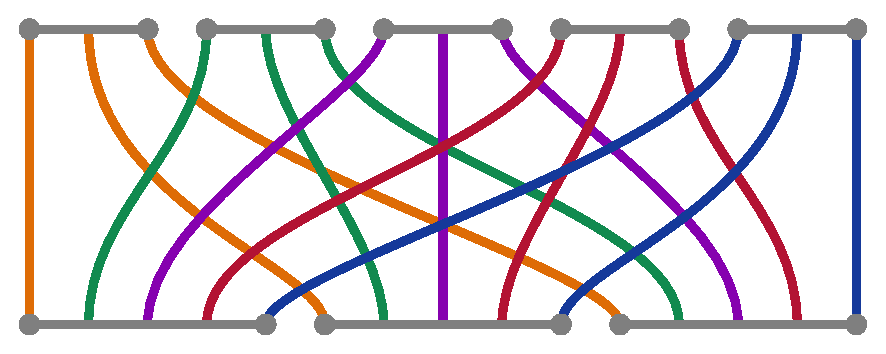
\includegraphics[width=0.8\columnwidth]{4-monoidal_structures/t-5-3.pdf}
\end{figure}
% We now give sufficient conditions for equipping the $2$-monad $\underline{P}$ associated to a $\Lambda$-operad $P$ with a pseudo-commutative structure. Let $\mathbb{N}_{+}$ denote the set of positive natural numbers.

We now define what it means for a $\Lambda$-operad to be pseudo-commuative, before then showing that such an operad yields a pseudo-commutative structure on the corresponding $2$-monad $\underline{P}$. Let $\mathbb{N}_{+}$ denote the set of positive integers.

QQQ Rewrite all this using the beta and delta operations, so it's consistent with before.
\begin{Defi}\label{def:ps-comm_operad}
Let $P$ be a $\Lambda$-operad. A pseudo-commutative structure on $P$ consists of:
    \begin{itemize}
        \item For each pair $(m,n) \in \mathbb{N}_{+}^2$, an element $t_{m,n} \in \Lambda(mn)$ such that $\pi(t_{m,n}) = \tau_{m,n}$.
        \item For each $p \in P(n)$, $q \in P(m)$, a natural isomorphism
            \[
                \lambda_{p,q} \colon \mu(p;q,\ldots,q) \cdot t_{m,n} \cong \mu(q;p,\ldots,p).
            \]
            We write this as $\lambda_{p,q}\colon \mu(p; \underline{q}) \cdot t_{m,n} \cong \mu(q; \underline{p})$.
    \end{itemize}
These are required to satisfy the following axioms:  
    \begin{enumerate}
        \item\label{axiom:t_id} For all $n \in \mathbb{N}_+$,
            \[
                t_{1,n} = e_n = t_{n,1}
            \]
             and for all $p \in P(n)$, the isomorphism $\lambda_{p, \id}\colon p \cdot e_n \cong p$ is the identity map.
        % \item\label{axiom:t_equiv} QQQ Equivariance axiom - we decided this was just naturality in the end! (See Remark 11.2 in \cite{guillou_multiplicative}.) QQQ It's basically `compose, act, switch' is the same as `compose, switch, act', but can't actually see where it's used in the proof:
        %   \[
        %     \lambda_{p \cdot g, q \cdot h} \circ \mu^P\left(\id_p \cdot g; \underline{\id_q \cdot h}\right) = \mu^P\left(\id_q \cdot h; \underline{\id_p \cdot g}\right) \circ \lambda_{p,q}.
        %   \]
        % For each $p \in P(n)$, $q \in P(m)$, $g \in \Lambda(n)$, and $h \in \Lambda(m)$, the following diagram commutes:
        %   \[
        %     \xy
        %       (-20,10)*+{\mu^P\left(p;\underline{q}\right) \cdot t_{m,n}}="a";
        %       (20,10)*+{\mu^P\left(q;\underline{p}\right)}="b";
        %       (-20,-10)*+{\mu^P\left(p \cdot g; \underline{q \cdot h}\right) \cdot t_{m,n}}="c";
        %       (20,-10)*+{\mu^P\left(q \cdot h; \underline{p \cdot g}\right)}="d";
        %       %
        %       {\ar^{\lambda_{p,q}} "a" ; "b"};
        %       {\ar^{\mu^P\left(\id_q \cdot h; \underline{\id_p \cdot g}\right)} "b" ; "d"};
        %       {\ar_{\mu^P\left(\id_p \cdot g; \underline{\id_q \cdot h}\right) \cdot t_{m,n}} "a" ; "c"};
        %       {\ar_{\lambda_{p \cdot g, q \cdot h}} "c" ; "d"};
        %     \endxy
        %   \]
        \item\label{axiom:t_sumR} For all $l, m_1, \ldots, m_l, n \in \mathbb{N}_+$, with $M = \Sigma m_i$,
            \[
                \mu^{\Lambda}\left(e_l; t_{m_1,n}, \ldots, t_{m_l,n}\right) \cdot \mu^{\Lambda}\left(t_{l,n};\underline{e_{m_1},\ldots,e_{m_l}}\right) = t_{n,M}.
            \]
            QQQ New version:
            \[
              \beta(t_{n,m_1},\ldots,t_{n,m_l}) \cdot \delta_{\underline{m_i},\ldots,\underline{m_i}}(t_{n,l}) = t_{n,M}.
            \]
            Here $\underline{e_{m_1},\ldots,e_{m_l}}$ is the list $e_{m_{1}}, \ldots, e_{m_{l}}$ repeated $n$ times.
        \item\label{axiom:t_sumL} For all $l, m, n_1,\ldots, n_m \in \mathbb{N}_+$, with $N = \Sigma n_i$,
            \[
                \mu^{\Lambda}\left(t_{m,l};\underline{e_{n_1}},\ldots,\underline{e_{n_m}}\right) \cdot \mu^{\Lambda}\left(e_m;t_{n_1,l},\ldots,t_{n_m,l}\right) = t_{N,l}.
            \]
            QQQ New version
            \[
              \delta_{\underline{n_1},\ldots,\underline{n_m}}(t_{m,l}) \cdot \beta(t_{n_1,l},\ldots,t_{n_m,l}) = t_{N,l}.
            \]
            Here $\underline{e_{n_{i}}}$ indicates that each $e_{n_{i}}$ is repeated $l$ times.
        \item\label{axiom:t_diagR} For any $l, m_i, n \in \mathbb{N}_+$, with $1 \leq i \leq n$, and $p \in P(l)$, $q_i \in P(m_i)$ and $r \in P(n)$, the following diagram commutes. (Note that we maintain the convention that anything underlined indicates a list, and double underlining indicates a list of lists. Each instance should have an obvious meaning from context and the equations appearing above.)
          \[
            \xy
                (0,0)*+{\mu\left(p;\underline{\mu(q_i;\underline{r})}\right) \cdot \mu(e_l;\underline{t_{n,m_i}})\mu(t_{n,l};\underline{\underline{e_{m_i}}})}="00";
                (60,0)*+{\mu\left(p;\underline{\mu(q_i;\underline{r})}\right) \cdot t_{n,M}}="10";
                (0,-15)*+{\mu\left(p;\underline{\mu(q_i;\underline{r})\cdot t_{n,m_i}}\right) \cdot \mu(t_{n,l};\underline{e_{m_1},\ldots,e_{m_l}})}="01";
                (60,-20)*+{\mu\left(\mu(p;q_1,\ldots,q_n);\underline{\underline{r}}\right)\cdot t_{n,M}}="11";
                (0,-30)*+{\mu\left(p;\underline{\mu(r;\underline{q_i})}\right) \cdot \mu(t_{n,l};\underline{e_{m_1},\ldots,e_{m_l}})}="02";
                (60,-40)*+{\mu\left(\mu(p;q_1,\ldots,q_n);\underline{\underline{r}}\right)}="12";
                (0,-45)*+{\mu\left(\mu(p;\underline{r}) \cdot t_{n,l} ; \underline{q_1,\ldots,q_n}\right)}="03";
                (60,-60)*+{\mu\left(r;\underline{\mu(p;q_1,\ldots,q_n)}\right)}="13";
                (0,-60)*+{\mu\left(\mu(r;\underline{p});\underline{q_1,\ldots,q_n}\right)}="04";
                {\ar@{=} "00" ; "10"};
                {\ar@{=} "00" ; "01"};
                {\ar@{=} "10" ; "11"};
                {\ar_{\mu(1;\underline{\lambda_{q_i,r}}) \cdot 1} "01" ; "02"};
                {\ar@{=} "02" ; "03"};
                {\ar@{=} "04" ; "13"};
                {\ar_{\mu(\lambda_{p,r};1)} "03" ; "04"};
                {\ar^{\lambda_{\mu(p;q_1,\ldots,q_n),r}} "11" ; "12"};
                {\ar@{=} "12" ; "13"};
            \endxy
          \]
        \item\label{axiom:t_diagL} For any $l,m, n_i \in \mathbb{N}_+$, with $1 \leq i \leq m$, and $p \in P(l)$, $q \in P(m)$ and $r_i \in P(n_i)$, the following diagram commutes.
          \[
            \xy
                (0,0)*+{\mu\left(\mu(p;\underline{q}) \cdot t_{m,l} ; \underline{\underline{r_i}}\right) \cdot \mu(e_m;\underline{t_{n_i,l}})}="00";
                (60,0)*+{\mu\left(\mu(p;\underline{q});\underline{\underline{r_i}}\right) \cdot \mu(t_{m,l};\underline{\underline{e_{n_i}}})\mu(e_{m};\underline{t_{n_i,l}})}="10";
                (60,-15)*+{\mu\left(p;\underline{\mu(q;\underline{r_i})}\right) \cdot \mu(t_{m,l};\underline{\underline{e_{n_i}}})\mu(e_{m};\underline{t_{n_i,l}})}="11";
                (0,-20)*+{\mu\left(\mu(q;\underline{p}); \underline{r_1},\ldots,\underline{r_m}\right) \cdot \mu(e_m;\underline{t_{n_i,l}})}="01";
                (0,-40)*+{\mu\left(q;\underline{\underline{\mu(p;r_i)}}\right) \cdot \mu(e_m;\underline{t_{n_i,l}})}="02";
                (0,-60)*+{\mu\left(q;\underline{\mu(p;\underline{r_i}) \cdot t_{n_i,l}}\right)}="03";
                (60,-30)*+{\mu\left(p;\underline{\mu(q;r_1,\ldots,r_m)}\right) \cdot t_{N,l}}="12";
                (60,-45)*+{\mu\left(\mu(q;r_1,\ldots,r_m); \underline{\underline{p}}\right)}="13";
                (60,-60)*+{\mu\left(q;\underline{\mu(r_i;\underline{p})}\right)}="14";
                {\ar@{=} "00" ; "10"};
                {\ar@{=} "10" ; "11"};
                {\ar@{=} "11" ; "12"};
                {\ar^{\lambda_{p,\mu(q;r_1,\ldots,r_m)}} "12" ; "13"};
                {\ar@{=} "13" ; "14"};
                {\ar_{\mu(\lambda_{p,q};1) \cdot 1} "00" ; "01"};
                {\ar@{=} "01" ; "02"};
                {\ar@{=} "02" ; "03"};
                {\ar_{\mu(1;\underline{\lambda_{p,r_i}})} "03" ; "14"};
            \endxy
          \]
    \end{enumerate}
\end{Defi}

\begin{remark}
Remark 11.2 of \cite{guillou_multiplicative} describes the need for an extra equivariance axiom in the pseudo-commutative structure definition, some detail of which is also described in \cite{guillou_symmetric}. We also believed this to be true until a realisation that the equivariance axiom of \cite{guillou_multiplicative}[11.1, Axiom (iii)] becomes the following requirement:
          \[
            \lambda_{p \cdot g, q \cdot h} \circ \left(\mu^P\left(\id_p \cdot g; \underline{\id_q \cdot h}\right) \cdot t_{m,n}\right) = \mu^P\left(\id_q \cdot h; \underline{\id_p \cdot g}\right) \circ \lambda_{p,q}.
          \]
On closer inspection, this appears to be an instance of naturality for the natural isomorphisms $\lambda$, as shown in the naturality square below.
          \[
            \xy
              (-20,10)*+{\mu^P\left(p;\underline{q}\right) \cdot t_{m,n}}="a";
              (20,10)*+{\mu^P\left(q;\underline{p}\right)}="b";
              (-20,-10)*+{\mu^P\left(p \cdot g; \underline{q \cdot h}\right) \cdot t_{m,n}}="c";
              (20,-10)*+{\mu^P\left(q \cdot h; \underline{p \cdot g}\right)}="d";
              %
              {\ar^{\lambda_{p,q}} "a" ; "b"};
              {\ar^{\mu^P\left(\id_q \cdot h; \underline{\id_p \cdot g}\right)} "b" ; "d"};
              {\ar_{\mu^P\left(\id_p \cdot g; \underline{\id_q \cdot h}\right) \cdot t_{m,n}} "a" ; "c"};
              {\ar_{\lambda_{p \cdot g, q \cdot h}} "c" ; "d"};
            \endxy
          \]
\end{remark}

\begin{thm}\label{pscomm}
Let $P$ be a $\Lambda$-operad equipped with a pseudo-commutative structure. Then $\underline{P}$ has a pseudo-commutativity.
\end{thm}

% \begin{thm}\label{pscomm}
% Let $P$ be a $\Lambda$-operad. Then the following equip $\underline{P}$ with a pseudo-commutative structure.
%     \begin{itemize}
%         \item For each pair $(m,n) \in \mathbb{N}_{+}^2$, we are given an element $t_{m,n} \in \Lambda(mn)$ such that $\pi(t_{m,n}) = \tau_{m,n}$.
%         \item For each $p \in P(n)$, $q \in P(m)$, we are given a natural isomorphism
%             \[
%                 \lambda_{p,q} \colon \mu(p;q,\ldots,q) \cdot t_{m,n} \cong \mu(q;p,\ldots,p).
%             \]
%             We write this as $\lambda_{p,q}\colon \mu(p; \underline{q}) \cdot t_{m,n} \cong \mu(q; \underline{p})$.
%     \end{itemize}
% These must satisfy the following:  
%     \begin{enumerate}
%         \item For all $n \in \mathbb{N}_+$\nomenclature[N]{$\mathbb{N}_+$}{the set of positive natural numbers},
%             \[
%                 t_{1,n} = e_n = t_{n,1}
%             \]
%              and for all $p \in P(n)$, the isomorphism $\lambda_{p, \id}\colon p \cdot e_n \cong p$ is the identity map.
%         \item For all $l, m_1, \ldots, m_l, n \in \mathbb{N}_+$, with $M = \Sigma m_i$,
%             \[
%                 \mu^{\Lambda}\left(e_l; t_{m_1,n}, \ldots, t_{m_l,n}\right) \cdot \mu^{\Lambda}\left(t_{l,n};\underline{e_{m_1},\ldots,e_{m_l}}\right) = t_{n,M}.
%             \]
%             Here $\underline{e_{m_1},\ldots,e_{m_l}}$ is the list $e_{m_{1}}, \ldots, e_{m_{l}}$ repeated $n$ times.
%         \item For all $l, m, n_1,\ldots, n_m \in \mathbb{N}_+$, with $N = \Sigma n_i$,
%             \[
%                 \mu^{\Lambda}\left(t_{m,l};\underline{e_{n_1}},\ldots,\underline{e_{n_m}}\right) \cdot \mu^{\Lambda}\left(e_m;t_{n_1,l},\ldots,t_{n_m,l}\right) = t_{N,l}.
%             \]
%             Here $\underline{e_{n_{i}}}$ indicates that each $e_{n_{i}}$ is repeated $l$ times.
%         \item For any $l, m_i, n \in \mathbb{N}_+$, with $1 \leq i \leq n$, and $p \in P(l)$, $q_i \in P(m_i)$ and $r \in P(n)$, the following diagram commutes. (Note that we maintain the convention that anything underlined indicates a list, and double underlining indicates a list of lists. Each instance should have an obvious meaning from context and the equations appearing above.)
%           \[
%             \xy
%                 (0,0)*+{\mu\left(p;\underline{\mu(q_i;\underline{r})}\right) \cdot \mu(e_l;\underline{t_{n,m_i}})\mu(t_{n,l};\underline{\underline{e_{m_i}}})}="00";
%                 (60,0)*+{\mu\left(p;\underline{\mu(q_i;\underline{r})}\right) \cdot t_{n,M}}="10";
%                 (0,-15)*+{\mu\left(p;\underline{\mu(q_i;\underline{r})\cdot t_{n,m_i}}\right) \cdot \mu(t_{n,l};\underline{e_{m_1},\ldots,e_{m_l}})}="01";
%                 (60,-20)*+{\mu\left(\mu(p;q_1,\ldots,q_n);\underline{\underline{r}}\right)\cdot t_{n,M}}="11";
%                 (0,-30)*+{\mu\left(p;\underline{\mu(r;\underline{q_i})}\right) \cdot \mu(t_{n,l};\underline{e_{m_1},\ldots,e_{m_l}})}="02";
%                 (60,-40)*+{\mu\left(\mu(p;q_1,\ldots,q_n);\underline{\underline{r}}\right)}="12";
%                 (0,-45)*+{\mu\left(\mu(p;\underline{r}) \cdot t_{n,l} ; \underline{q_1,\ldots,q_n}\right)}="03";
%                 (60,-60)*+{\mu\left(r;\underline{\mu(p;q_1,\ldots,q_n)}\right)}="13";
%                 (0,-60)*+{\mu\left(\mu(r,\underline{p});\underline{q_1,\ldots,q_n}\right)}="04";
%                 {\ar@{=} "00" ; "10"};
%                 {\ar@{=} "00" ; "01"};
%                 {\ar@{=} "10" ; "11"};
%                 {\ar_{\mu(1;\underline{\lambda_{q_i,r}}) \cdot 1} "01" ; "02"};
%                 {\ar@{=} "02" ; "03"};
%                 {\ar@{=} "04" ; "13"};
%                 {\ar_{\mu(\lambda_{p,r};1)} "03" ; "04"};
%                 {\ar^{\lambda_{\mu(p;q_1,\ldots,q_n),r}} "11" ; "12"};
%                 {\ar@{=} "12" ; "13"};
%             \endxy
%           \]
%         \item For any $l,m, n_i \in \mathbb{N}_+$, with $1 \leq i \leq m$, and $p \in P(l)$, $q \in P(m)$ and $r_i \in P(n_i)$, the following diagram commutes.
%           \[
%             \xy
%                 (0,0)*+{\mu\left(\mu(p;\underline{q}) \cdot t_{m,l} ; \underline{\underline{r_i}}\right) \cdot \mu(e_m;\underline{t_{n_i,l}})}="00";
%                 (60,0)*+{\mu\left(\mu(p;\underline{q});\underline{\underline{r_i}}\right) \cdot \mu(t_{m,l};\underline{\underline{e_{n_i}}})\mu(e_{m};\underline{t_{n_i,l}})}="10";
%                 (60,-15)*+{\mu\left(p;\underline{\mu(q;\underline{r_i})}\right) \cdot \mu(t_{m,l};\underline{\underline{e_{n_i}}})\mu(e_{m};\underline{t_{n_i,l}})}="11";
%                 (0,-20)*+{\mu\left(\mu(q;\underline{p}); \underline{r_1},\ldots,\underline{r_m}\right) \cdot \mu(e_m;\underline{t_{n_i,l}})}="01";
%                 (0,-40)*+{\mu\left(q;\underline{\underline{\mu(p;r_i)}}\right) \cdot \mu(e_m;\underline{t_{n_i,l}})}="02";
%                 (0,-60)*+{\mu\left(q;\underline{\mu(p;\underline{r_i}) \cdot t_{n_i,l}}\right)}="03";
%                 (60,-30)*+{\mu\left(p;\underline{\mu(q;r_1,\ldots,r_m)}\right) \cdot t_{N,l}}="12";
%                 (60,-45)*+{\mu\left(\mu(q;r_1,\ldots,r_m); \underline{\underline{p}}\right)}="13";
%                 (60,-60)*+{\mu\left(q;\underline{\mu(r_i;\underline{p})}\right)}="14";
%                 {\ar@{=} "00" ; "10"};
%                 {\ar@{=} "10" ; "11"};
%                 {\ar@{=} "11" ; "12"};
%                 {\ar^{\lambda_{p,\mu(q;r_1,\ldots,r_m)}} "12" ; "13"};
%                 {\ar@{=} "13" ; "14"};
%                 {\ar_{\mu(\lambda_{p,q};1) \cdot 1} "00" ; "01"};
%                 {\ar@{=} "01" ; "02"};
%                 {\ar@{=} "02" ; "03"};
%                 {\ar_{\mu(1;\underline{\lambda_{p,r_i}})} "03" ; "14"};
%             \endxy
%           \]
%     \end{enumerate}
% \end{thm}

\begin{proof}
We refer to the Axioms in \cref{def:ps-comm_operad} throughout. We begin the proof by defining an invertible modification $\gamma$ for the pseudo-commutativity for which the components are natural transformations $\gamma_{A,B}$. Such a transformation $\gamma_{A,B}$ has components with source
  \[
    \left[\mu\left(p; \underline{q}\right); \underline{(a, \underline{b})}\right]
  \]
and target
  \[
    \left[\mu\left(q; \underline{p}\right); \underline{(\underline{a},b)}\right].
  \]
Now $ \lambda_{p,q} \colon \mu(p;q,\ldots,q) \cdot t_{m,n} \cong \mu(q;p,\ldots,p)$ gives rise to another map by multiplication on the right by $t_{m,n}^{-1}$,
  \[
    \lambda_{p,q}\cdot t_{m,n}^{-1} \colon \mu(p;q,\ldots,q) \cong \mu(q;p,\ldots,p) \cdot t_{m,n}^{-1},
  \]
so we define $(\gamma_{A,B})_{[p;a_1,\ldots,a_n],[q;b_1,\ldots,b_m]}$ to be the morphism which is the image of $(\lambda_{p,q}\cdot t_{m,n}^{-1}, 1)$ under the map
  \[
    \coprod P(n) \times (A \times B)^{n} \rightarrow \coprod P(n) \times_{\Lambda(n)} (A \times B)^{n}.
  \]
Naturality of $\gamma_{A,B}$ follows from that of each $\lambda_{p,q}$. We will write this morphism as $[\lambda_{p,q}t_{m,n}^{-1}, 1]$. In the case that either $p$ or $q$ is an identity then we choose the component of $\gamma$ to be the isomorphism involving the appropriate identity element using Axiom \ref{axiom:t_id} above.

There are two things to note about the definition above before we continue. First, it is easy to check that
  \[
    t_{m,n}^{-1} \cdot \underline{\left(a, \underline{b}\right)} = \underline{\left(\underline{a},b\right)}
  \]
since $\pi(t_{m,n}) = \tau_{m,n}$; this ensures that $\gamma$ has the correct target. Second, the morphism above has second component the identity. This is actually forced upon us by the requirement that $\gamma$ be a modification:  in the case that $A,B$ are discrete categories, the only possible morphism is an identity, and the modification axiom then forces that statement to be true for general $A,B$ by considering the inclusion $A_{0} \times B_{0} \hookrightarrow A \times B$ where $A_{0}, B_{0}$ are the discrete categories with the same objects as $A, B$.

We show that this is a modification by noting that it does not rely on objects in the lists $a_1, \ldots, a_n$ or $b_1, \ldots, b_m$, only on their lengths and the operations $p$ and $q$. As a result, if there are functors $f \colon A \rightarrow A'$ and $g \colon B \rightarrow B'$, then it is clear that
    \[
        (\underline{P}(f\times g) \circ \gamma_{A,B})_{\left[p;\underline{a}\right],\left[q;\underline{b}\right]} = [\lambda_{p,q},\underline{1}] = (\gamma_{A',B'} \circ (\underline{P}f\times \underline{P}g))_{\left[p;\underline{a}\right],\left[q;\underline{b}\right]}.
    \]
As such we can simply write $(\gamma_{A,B})_{[p;\underline{a}],[q;\underline{b}]}$ in shorthand as $\gamma_{p,q}$.

There are now seven axioms to check for a pseudo-commutativity:  three strength axioms, two unit axioms, and two multiplication axioms. For the first strength axiom, we must verify that two different $2$-cells of shape
  \[
    \xy
      (0,0)*+{A \times TB \times TC}="0";
      (50,0)*+{T(A \times B \times C)}="1";
      {\ar@/^1pc/ "0"; "1"};
      {\ar@/_1pc/ "0"; "1"};
      (25,0)*{\Downarrow}
    \endxy
  \]
are equal. The first of these is $\gamma$ precomposed with $d \times 1$, and so is the component of $\gamma$ at an object
  \[
    \left( [p;(a,b_1),\ldots,(a,b_n)], [q; c_{1}, \ldots, c_{m}] \right).
  \]
The second of these is $d$ applied to the component of $1 \times \gamma$ at
  \[
    \left(a, ([p;b_1,\ldots,b_n], [q; c_{1}, \ldots, c_{m}]) \right).
  \]
It is straightforward to compute that each of these maps is the image of $\left(\lambda_{p,q}\cdot t_{m,n}^{-1},1\right)$ under the functor
  \[
    \coprod P(n) \times (A \times B)^{n} \rightarrow \coprod P(n) \times_{\Lambda(n)} (A \times B)^{n}.
  \]
The other two strength axioms follow by analogous calculations for other whiskerings of $\gamma$ with $d$ or $d^{*}$.

For the unit axioms, we must compute the components of $\gamma$ precomposed with $\eta \times 1$ for the first axiom and $1 \times \eta$ for the second. Thus for the first unit axiom, we must compute the component of $\gamma$ at $\left( [e;a], [p; b_{1}, \ldots, b_{m}] \right)$. By definition, this is the image of $(\lambda_{e,p}\cdot t^{-1}_{m,1}, 1)$ under the map to the coequalizer, and by Axiom \ref{axiom:t_id} of \ref{def:ps-comm_operad} know that $t^{-1}_{m,1}$ is the identity element and this isomorphism is the identity as well, so this component of $\gamma$ is also the identity. The second unit axiom follows similarly, using that $t^{-1}_{1,n}$ is the identity.

For the multiplication axioms, first note that Axiom \ref{axiom:t_sumR} is necessary in order to ensure the existence of the top horizontal equality in the diagram of Axiom \ref{axiom:t_diagR} for the pseudo-commutative structure; the same goes for Axioms \ref{axiom:t_sumL} and \ref{axiom:t_diagL}. We now explain how Axioms \ref{axiom:t_sumR} and \ref{axiom:t_diagR} for the pseudo-commutative structure ensure that the first multiplication axiom holds, with the same reasoning showing that Axioms \ref{axiom:t_sumL} and \ref{axiom:t_diagL} imply the second multiplication axiom.

We begin by studying the pasting diagram in the first multiplication axiom, but computing its values using the strength and costrength for the non-symmetric operad underlying $P$; this means that we evaluate on objects of the form $(p; a_{1}, \ldots, a_{n})$ rather than on their equivalence classes. Let $p \in P(l), q_{i} \in P(m_{i})$ for $1 \leq i \leq l$, and $r \in P(n)$. Computing the top and right leg around the pasting diagram gives the function on objects which sends
  \[
    \left( (p; (q_{1}; \un{a_{1}}), \ldots, (q_{l}; \un{a_{l}})), (r; \un{b}) \right)
  \]
to
  \[
    \left( \mu(p; \mu(q_{1}; \un{r}), \ldots, \mu(q_{l}; \un{r})); (\un{(a_{1\bullet}, \un{b})}), \ldots, (\un{(a_{l\bullet}, \un{b})}) \right),
  \]
where $(\un{(a_{i\bullet}, \un{b})})$ is the list of pairs
  \[
    (a_{i1}, b_{1}), \ldots, (a_{i1}, b_{m}), (a_{i2}, b_{1}), \ldots, (a_{in_{i}}, b_{m}).
  \]
Then $\un{P}\gamma$ is the image of the morphism which is the identity on the $(a_{ij}, b_{k})$'s, and is the morphism
  \[
    \mu\left(1;\lambda_{q_1,r}t^{-1}_{n,m_1},\ldots,\lambda_{q_l,r}t^{-1}_{n,m_l}\right)
  \]
on the first component with domain and codomain shown below.
  \[
    \mu\left(p;\mu\left(q_1;\un{r}\right),\ldots,\mu\left(q_n;\un{r}\right)\right) \longrightarrow \mu\left(p;\mu\left(r;\un{q_1}\right)t^{-1}_{n,m_1},\ldots,\mu\left(r;\un{q_l}\right)t^{-1}_{n,m_l}\right)
  \]
% \[
% \xy
% {\ar^{\scriptstyle \mu\left(1; \lambda_{q_{1}, r} t^{-1}_{n,m_{1}}, \ldots, \lambda_{q_{1}, r} t^{-1}_{n,m_{l}}\right)} (0,0)*+{\scriptstyle \mu\left(p; \mu(q_{1}; \un{r}), \ldots, \mu(q_{n}; \un{r})\right)}; (75,0)*+{\scriptstyle \mu\left(p; \mu(r; \un{q_{1}}) t^{-1}_{n,m_{1}}, \ldots, \mu(r; \un{q_{l}}) t^{-1}_{n,m_{l}} \right)} }
% \endxy
% \]
% on the first component. 
By the $\Lambda$-operad axioms, the target of this morphism is equal to
  \[
    \mu\left(p; \mu\left(r; \un{q_{1}}\right), \ldots, \mu\left(r; \un{q_{l}}\right) \right)\mu\left(e_{l}; t^{-1}_{n,m_{1}}, \ldots, t^{-1}_{n,m_{l}}\right).
  \]
Note that this is not the same object as one obtains by computing $T\mu \circ T^{2}d^{*} \circ Td \circ d^{*}$ using the underlying non-symmetric operad of $P$ as we are required to use the $\Lambda$-equivariance to ensure that the target of $\gamma$ is the correct one.

Next we compute the source of $(\mu \circ Td^{*})*\gamma$, the other $2$-cell in the pasting appearing in the first multiplication axiom. We compute this once again using the strength and costrength for the underlying non-symmetric operad, and note once again that this will not match our previous calculations precisely, but only up to an application of $\Lambda$-equivariance. This functor has its map on objects given by
  \[
    \left( (p; (q_{1}; \un{a_{1}}), \ldots, (q_{l}; \un{a_{l}})), (r; \un{b}) \right) \mapsto \left(\mu(\mu(p; \un{r}); \un{q_{1}}, \ldots, \un{q_{l}}); \un{(\un{a_{1}}, b_{\bullet})}, \ldots, \un{(\un{a_{l}}, b_{\bullet})} \right).
  \]
  Note that if we apply $\Lambda$-equivariance, this matches the target computed above. Once again the component of $\gamma$ is the image of a morphism which is the identity on the $(a_{ij}, b_{k})$'s, and its first component is
  \[
    \xy
      {\ar^{\mu\left(\lambda_{p,r} \cdot t^{-1}_{n,l}; 1, \ldots, 1\right)} (0,0)*+{\mu\left(\mu(p; \un{r}); \un{q_{1}}, \ldots, \un{q_{l}}\right)}; (60,0)*+{\mu\left(\mu(r; \un{p})\cdot t^{-1}_{n,l}; \un{q_{1}}, \ldots, \un{q_{l}}\right).} }
    \endxy
  \]

We cannot compose these morphisms in $\coprod P(n) \times (A \times B)^{n}$ as they do not have matching source and target, but we can in $\coprod P(n) \times_{\Lambda} (A \times B)^{n}$. The resulting morphism has first component given by the image of
  \[
    \xy
      {\ar^{\scriptstyle \mu\left(1; \lambda_{q_{1}, r} t^{-1}_{n,m_{1}}, \ldots, \lambda_{q_{1}, r} t^{-1}_{n,m_{l}}\right)} (0,0)*+{\scriptstyle \mu\left(p; \mu\left(q_{1}; \un{r}\right), \ldots, \mu\left(q_{n}; \un{r}\right)\right)}; (75,0)*+{\scriptstyle \mu\left(p; \mu\left(r; \un{q_{1}}\right) t^{-1}_{n,m_{1}}, \ldots, \mu\left(r; \un{q_{l}}\right) t^{-1}_{n,m_{l}} \right)} };
      {\ar^<<<<<<<<<<<<<<<<<<<<<<{\scriptstyle \mu\left(\lambda_{p,r} \cdot t^{-1}_{n,l}; 1, \ldots, 1\right)\cdot \mu\left(e_{l}; t^{-1}_{n,m_{1}}, \ldots, t^{-1}_{n,m_{l}}\right)} (0,-10)*+{}; (75,-10)*+{\scriptstyle \mu\left(\mu\left(r; \un{p}\right)\cdot t^{-1}_{n,l}; \un{q_{1}}, \ldots, \un{q_{l}}\right)\cdot \mu\left(e_{l}; t^{-1}_{n,m_{1}}, \ldots, t^{-1}_{n,m_{l}}\right),} }
    \endxy
  \]
where we have made use of the operad axioms in identifying the target of the first map with the source of the second. Using the $\Lambda$-operad axioms again on the target, we find that
  \[
    \mu\left(\mu(r; \un{p})\cdot t^{-1}_{n,l}; \un{q_{1}}, \ldots, \un{q_{l}}\right)\cdot \mu(e_{l}; t^{-1}_{n,m_{1}}, \ldots, t^{-1}_{n,m_{l}})
  \]
is equal to
  \[
    \mu\left(\mu(r; \un{p}); \un{q_{1}, \ldots, q_{l}}\right) \cdot \mu(t^{-1}_{n,l}; \un{e}) \cdot \mu(e_{l}; t^{-1}_{n,m_{1}}, \ldots, t^{-1}_{n,m_{l}}).
  \]
This composite of two morphisms, together with the necessary identities coming from operad axioms, is precisely the left and bottom leg of the diagram in Axiom \ref{axiom:t_diagR}. Using the same method, one then verifies that $\gamma * (\mu \times 1)$ has its first component the image of the morphism appearing along the top and right leg of the diagram in \ref{axiom:t_diagR}. The second component of these morphisms are all identities arising from $\Lambda$-equivariance, so the first multiplication axiom is a consequence of Axioms \ref{axiom:t_sumR} and \ref{axiom:t_diagR} for the pseudo-commutative structure. We leave the calculations for the second multiplication axiom to the reader as they are of the same nature, using Axioms \ref{axiom:t_sumL} and \ref{axiom:t_diagL}.
\end{proof}

\begin{cor}
Let $P$ be a non-symmetric operad. Then the induced monad $\underline{P}$ is never pseudo-commutative.
\end{cor}
\begin{proof}
In the non-symmetric case, the $2$-monad is just given using coproducts and products, i.e., there is no coequalizer. In order to define $\gamma$, we then need an isomorphism
  \[
    \left(\mu(p; \underline{q}); \underline{(a, \underline{b})}\right) \cong \left(\mu(q; \underline{p}); \underline{(\underline{a},b)}\right).
  \]
When $A,B$ are discrete, there is no isomorphism $\underline{\left(a,\underline{b}\right)} \cong \underline{\left(\underline{a},b\right)}$, and therefore no such $\gamma$ can exist.
\end{proof}



A further property that a pseudo-commutativity can possess is that of symmetry. This symmetry is then reflected in the monoidal structure on the $2$-category of algebras, which will then also have a symmetric tensor product (in a suitable, $2$-categorical sense).

\begin{Defi}
Let $T \colon \m{K} \rightarrow \m{K}$ be a $2$-monad on a symmetric monoidal $2$-category $\m{K}$ with symmetry $c$. We then say that a pseudo-commutativity $\gamma$ for $T$ is \textit{symmetric} when the following is satisfied for all $A$, $B \in \m{K}$:
    \[
        Tc_{A,B} \circ \gamma_{A,B} \circ c_{TB, TA} = \gamma_{B,A}.
    \]
\end{Defi}

With the notion of symmetry at hand we are able to extend the above theorem, stating when $\underline{P}$ is symmetric.
\begin{thm}
The pseudo-commutativity of $\underline{P}$ given by \cref{pscomm}  is symmetric if for all $m,n \in \mathbb{N}_+$ the two conditions below hold.
    \begin{enumerate}
        \item $t_{m,n} = t_{n,m}^{-1}$.
        \item The following diagram commutes:
          \[
              \xy
                (0,0)*+{\mu\left(p;\underline{q}\right) \cdot t_{m,n}t_{n,m}}="00";
                (30,0)*+{\mu\left(p;\underline{q}\right) \cdot e_{mn}}="10";
                (0,-15)*+{\mu\left(q;\underline{p}\right) \cdot t_{n,m}}="01";
                (30,-15)*+{\mu\left(p;\underline{q}\right)}="11";
                {\ar@{=} "00" ; "10"};
                {\ar_{\lambda_{p,q} \cdot 1} "00" ; "01"};
                {\ar@{=} "10" ; "11"};
                {\ar_{\lambda_{q,p}} "01" ; "11"};
              \endxy
          \]
    \end{enumerate}
\end{thm}
\begin{proof}
The commutativity of the diagram above ensures that the first component of the symmetry axiom commutes in $P(n)$ before taking equivalence classes in the coequalizer, just as in the proof of \cref{pscomm}.
\end{proof}

\begin{Defi}
Let $P$ be a $\Lambda$-operad in $\mb{Cat}$. We say that $P$ is \textit{contractible} if each category $P(n)$ is equivalent to the terminal category.
\end{Defi}

\begin{cor}
If $P$ is contractible and there exist $t_{m,n}$ as in \cref{pscomm}, then $\underline{P}$ acquires a pseudo-commutativity. Furthermore, it is symmetric if $t_{n,m} = t_{m,n}^{-1}$.
\end{cor}
\begin{proof}
The only thing left to define is the collection of natural isomorphisms $\lambda_{p,q}$. But since each $P(n)$ is contractible, $\lambda_{p,q}$ must be the unique isomorphism between its source and target, and furthermore the last two axioms hold since any pair of parallel arrows are equal in a contractible category.
\end{proof}

\begin{cor}
If $P$ is a contractible symmetric operad then $\underline{P}$ has a symmetric pseudo-commutativity.
\end{cor}
\begin{proof}
We choose $t_{m,n} = \tau_{m,n}$.
\end{proof}

\begin{rem}
If a $\Lambda$-operad $P$ is contractible, it is not the case that its symmetrization $S(P)$ (see \cref{thm_sym}) will also be contractible. The category $P(n) \times_{\Lambda(n)} \Sigma_{n}$ will necessarily be a groupoid as it is a colimit of groupoids: contractible categories are always groupoids, and both $\Lambda(n)$ and $\Sigma_{n}$ are discrete. Let $g \in \textrm{ker} \, \pi_{n}$ be any non-identity element, and let $p \in P(n)$ be any object. Then
  \[
    [p \cdot g, e] = [p, \pi(g)e] = [p,e],
  \]
but unless $p\cdot g = p$ in $P(n)$, there will be a unique isomorphism between them that will not be the identity, and hence will define a nontrivial automorphism of $[p,e]$ in  $P(n) \times_{\Lambda(n)} \Sigma_{n}$. The existence of such ensures that $P(n) \times_{\Lambda(n)} \Sigma_{n}$ is not contractible.
\end{rem}


We conclude with a computation using \cref{pscomm}. This result (\ref{braidpscomm} below) was only conjectured in \cite{HP}, but we are able to prove it quite easily with the machinery developed thus far. Our strategy is to construct a $\Lambda$-operad which is contractible together with the group elements required in \cref{pscomm}. Note that the symmetrized version of this operad will not be contractible, and we do not know of a proof using the structure of the symmetrized operad.

\begin{thm}\label{braidpscomm}
The $2$-monad $\underline{B}$ for braided strict monoidal categories on $\mb{Cat}$ has two pseudo-commutative structures on it, neither of which are symmetric.
\end{thm}

In order to apply our theory, the $2$-monad $\underline{B}$ must arise from a $\Lambda$-operad. The following proposition describes it as such, and can largely be found as Example 3.2 in the work of Fiedorowicz \cite{fie-br}.

\begin{prop}
The $2$-monad $\underline{B}$ is the $2$-monad associated to the $B$-operad $B$ with the category $B(n)$ having objects the elements of the $n$th braid group $B_{n}$ and a unique isomorphism between any pair of objects; the action of $B_{n}$ on $B(n)$ is given by right multiplication on objects and is then uniquely determined on morphisms.
\end{prop}

The interested reader could easily verify that algebras for the $B$-operad $B$ are braided strict monoidal categories. The objects of $\underline{B}(X)$ can be identified with finite lists of objects of $X$, and morphisms are generated by the morphisms of $X$ together with new isomorphisms
  \[
    x_{1}, \ldots, x_{n} \stackrel{\gamma}{\longrightarrow} x_{\gamma^{-1}(1)}, \ldots, x_{\gamma^{-1}(n)}
  \]
where $\gamma \in B_{n}$ and the notation $\gamma^{-1}(i)$ means, as before, that we take the preimage of $i$ under the permutation $\pi(\gamma)$ associated to $\gamma$. This shows that $\underline{B}(X)$ is the free braided strict monoidal category generated by $X$ according to \cite{js}, and it is easy to verify that the $2$-monad structure on $\underline{B}$ arising from the $B$-operad structure on $B$ is the correct one to produce braided strict monoidal categories as algebras.

\begin{Defi}
A braid $\gamma \in B_{n}$ is \textit{positive} if it is an element of the submonoid of $B_{n}$ generated by the elements $\sigma_{1}, \sigma_{2}, \ldots, \sigma_{n-1}$.
\end{Defi}

\begin{Defi}
 A braid $\gamma \in B_{n}$ is \textit{minimal} if no pair of strands in $\gamma$ cross twice.
\end{Defi}

For our purposes, we are interested in braids which are both positive and minimal. A proof of the following lemma can be found in \cite{EM2}.

\begin{lem}\label{pmlem}
Let $PM_{n}$ be the subset of $B_{n}$ consisting of positive, minimal braids. Then the function sending a braid to its underlying permutation is a bijection of sets $PM_{n} \rightarrow \Sigma_{n}$.
\end{lem}

\begin{rem}\label{pmrem}
It is worth noting that this bijection is not an isomorphism of groups, since $PM_{n}$ is not a group or even a monoid. The element $\sigma_{1} \in B_{n}$ is certainly in $PM_{n}$, but $\sigma_{1}^{2}$ is not as the first two strands cross twice. Thus we see that the product of two minimal braids is generally not minimal, but by definition the product of positive braids is positive.
\end{rem}

\begin{proof}[Proof of \cref{braidpscomm}]
We refer to the Axioms of \cref{def:ps-comm_operad} throughout the proof. In order to use \cref{pscomm} with the action operad being the braid operad $B$, we must first construct elements $t_{m,n} \in B_{mn}$ satisfying certain properties. Using \cref{pmlem}, we define $t_{m,n}$ to be the unique positive minimal braid such that $\pi(t_{m,n}) = \tau_{m,n}$. Since $\tau_{1,n} = e_{n} = \tau_{n,1}$ in $\Sigma_{n}$ and the identity element $e_{n} \in B_{n}$ is positive and minimal, we find that $t_{1,n} = e_{n} = t_{n,1}$ in $B_{n}$, satisfying Axiom \ref{axiom:t_id}. Thus in order to verify the remaining hypotheses, we must check two equations, each of which states that some element $t_{m,n}$ can be expressed as a product of operadic compositions of other elements.

Let $l, m_{1}, \ldots, m_{l}, n$ be natural numbers, and let $N = \sum m_{i}$. We must check Axiom \ref{axiom:t_sumL} is satisfied, i.e., that
  \[
    \beta(t_{n, m_{1}}, \ldots, t_{n, m_{l}}) \cdot \delta(t_{n,l}) = t_{N, l}
  \]
  \[
    \mu(e_{l}; t_{n, m_{1}}, \ldots, t_{n, m_{l}}) \mu\left(t_{n,l}; \underline{e_{m_{1}}, \ldots, e_{m_{l}}}\right) = t_{N, l}
  \]
in $B_{lN}$. These braids have the same underlying permutations by construction, and both are positive since each operadic composition on the left is positive. The braid on the right is minimal by definition, so if we prove that the braid on the left is also minimal, they are necessarily equal. Now $\mu\left(t_{n,l}; \underline{e_{m_{1}}, \ldots, e_{m_{l}}}\right)$ is given by the braid for $t_{n,l}$ but with the first strand replaced by $m_{1}$ strands, the second strand replaced by $m_{2}$ strands, and so on for the first $l$ strands of $t_{n,l}$, and then repeating for each group of $l$ strands. In particular, since strands $i, i+l, i+2l, \ldots, i + (n-1)l$ never cross in $t_{n,l}$, none of the $m_{i}$ strands that each of these is replaced with cross. The braid $\mu(e_{l}; t_{n, m_{1}}, \ldots, t_{n, m_{l}})$ consists of the disjoint union of the braids for each $t_{n,m_{i}}$, so if two strands cross in $\mu(e_{l}; t_{n, m_{1}}, \ldots, t_{n, m_{l}})$ then they must both cross in some $t_{n,m_{i}}$. The strands in $t_{n,m_{i}}$ are those numbered from $n(m_{1} + \cdots + m_{i-1}) + 1$ to $n(m_{1} + \cdots + m_{i-1} + m_{i})$. This is a consecutive collection of $nm_{i}$ strands, and it is simple to check that these strands are precisely those connected (via the group operation in $B_{Nl}$, concatenation) to the duplicated copies of strands $i, i+l, i+2l, \ldots, i + (n-1)l$ in $t_{n,l}$. Thus if a pair of strands were to cross in
% $\mu(e_{l}; t_{n, m_{1}}, \ldots, t_{n, m_{l}})$
$\beta(t_{n, m_{1}}, \ldots, t_{n, m_{l}})$, that pair cannot also have crossed in
% $\mu\left(t_{n,l}; \underline{e_{m_{1}}, \ldots, e_{m_{l}}}\right)$
$\delta(t_{n,l})$, showing that the resulting product braid
  \[
    \beta(t_{n, m_{1}}, \ldots, t_{n, m_{l}}) \cdot \delta(t_{n,l})
  \]
  \[
    \mu(e_{l}; t_{n, m_{1}}, \ldots, t_{n, m_{l}}) \mu\left(t_{n,l}; \underline{e_{m_{1}}, \ldots, e_{m_{l}}}\right)
  \]
is minimal. The calculation for Axiom \ref{axiom:t_sumR}, showing that
  \[
    \delta(t_{m,l}) \cdot \beta(t_{n_{1}, l}, \ldots, t_{n_{m}, l})
  \]
  \[
    \mu\left(t_{m,l}; \underline{e_{1}}, \ldots, \underline{e_{n_{m}}}\right) \mu\left(e_{m}; t_{n_{1}, l}, \ldots, t_{n_{m}, l}\right)
  \]
is also minimal, follows from the same argument, showing that it is equal to $t_{N, l}$ (here $N$ is the sum of the $n_{i}$, where once again $i$ ranges from 1 to $l$).

QQQ Where are Axioms \ref{axiom:t_diagR} and \ref{axiom:t_diagL} checked?

These calculations show, using \cref{pscomm}, that the $B$-operad $B$ induces a $2$-monad which has a pseudo-commutative structure. As noted before, $B$-algebras are precisely braided strict monoidal categories. The second pseudo-commutative structure arises by using negative, minimal braids instead of positive ones, and proceeds using the same arguments. This finishes the first part of the proof of \cref{braidpscomm}.

We will now show that neither of these pseudo-commutative structures is symmetric. The symmetry axiom in this case reduces to the fact that, in some category which is given as a coequalizer, the morphism with first component
  \[
    f\colon \mu\left(p; \underline{q}\right) \cdot t_{n,m}t_{m,n} \rightarrow \mu\left(q; \underline{p}\right) \cdot t_{m,n} \rightarrow \mu\left(p; \underline{q}\right)
  \]
is the identity. Now it is clear that $t_{n,m}$ is not equal to $t_{m,n}^{-1}$ in general: taking $m=n=2$, we note that $t_{2,2} = \sigma_{2}$, and this element is certainly not of order two in $B_{4}$. $B(4)$ is the category whose objects are the elements of $B_{4}$ with a unique isomorphism between any two pair of objects, and $B_{4}$ acts by multiplication on the right; this action is easily shown to be free and transitive. We recall (see \cref{coeq-lem}) that in a coequalizer of the form $A \times_{G} B$, a morphism $[f_{1}, f_{2}]$ equals $[g_{1}, g_{2}]$ if and only if there exists an $x \in G$ such that
  \begin{align*}
    f_{1} \cdot x &= g_{1}, \\
    x^{-1} \cdot f_{2} &= g_{2}.
  \end{align*}
For the coequalizer in question, for $f$ to be the first component of an identity morphism would imply that $f \cdot x$ would be a genuine identity in $B(4)$ for some $x$. But $f \cdot x$ would have source $\mu\left(p; \underline{q}\right) t_{n,m}t_{m,n}x$ and target $\mu\left(p; \underline{q}\right)x$, which requires $t_{n,m}t_{m,n}$ to be the identity group element for all $n,m$. In particular, this would force $t_{2,2}$ to have order two, which as noted above does not hold in $B_{4}$, thus giving a contradiction.
\end{proof}

\begin{rem}
The pseudo-commutativities given above are not necessarily the only ones that exist for the $B$-operad $B$, but we do not know a general strategy for producing others.
\end{rem}

\begin{example}
Non-Example: Cactus operad.

Begin by defining $t_{2,2} = s_{2,3}$, which has underlying permutation $\pi_4(t_{2,2}) = \trans{2}{3} = \tau_{2,3}$, as required. This seems to be a sensible choice to then demonstrate that we can describe all other $t_{m,n}$ required for a pseudo-commutativity on $J$. In particular, we should be able to describe $t_{2,4}$ which would have underlying permutation $\tau_{2,4} = (2 \,\, 3 \,\, 5)(4 \,\, 7 \,\, 6)$. If the required elements $t_{m,m}$ existed for the cactus operad $J$, then we would be able to apply the axioms from \cref{def:ps-comm_operad} to the element $t_{2,4}$ in order to see how it is constructed from $t_{2,2} = s_{2,3}$.

By Axiom \ref{axiom:t_sumR} of \cref{def:ps-comm_operad} we should be able to split the element $t_{2,4}$ up as follows.
  \begin{align*}
    t_{2,4} &= t_{2,2+2} \\
    &= \beta(t_{2,2},t_{2,2}) \cdot \delta_{2,2,2,2}(t_{2,2}) \\
    &= s_{2,3} \cdot s_{5,7} \cdot \delta_{2,2,2,2}(s_{2,3}) \\
    &= s_{2,3} \cdot s_{5,7} \cdot s_{2,6} \cdot \beta(e_2,s_{1,2},s_{1,2},e_2) \\
    &= s_{2,3} \cdot s_{5,7} \cdot s_{2,6} \cdot s_{3,4} \cdot s_{5,6}.
  \end{align*}
Here we have used $\delta$ as defined for generators $s_{p,q}$ in \cref{J_aop}. This element has underlying permutation
  \[
      \trans{2}{3}\trans{5}{7}\trans{2}{6}\trans{3}{5}\trans{3}{4}\trans{5}{6} = \trans{2}{6}(3 \,\, 4 \,\, 7 \,\,5)
  \]
which is not equal to $\tau_{2,4} = (2 \,\, 3 \,\, 5)(4 \,\, 7 \,\, 6)$. Hence if $J$ were to have a pseudo-commutative structure, then it cannot arise in this way.
\end{example}
\subsection{Profunctors and multicategories}
In this section we generalize from operads to multicategories (or colored operads). The notions of plain and symmetric multicategories are standard \cite{bd_hda3}, but in fact there is a corresponding notion of $\Lambda$-multicategory for any action operad $\Lambda$. We will give the basic definition and then show that it arises abstractly from a lifting of $\underline{E\Lambda}$ as a $2$-monad  on $\mb{Cat}$ to a pseudomonad on $\mb{Prof}$, the bicategory of categories, profunctors, and transformations. A quick treatment of similar material but restricted to the symmetric case can be found in \cite{garner_poly}.

\begin{Defi}\label{lambda_multicat}
Let $\Lambda$ be an action operad. A \emph{$\Lambda$-multicategory} $M$ consists of the following data:
\begin{itemize}
  \item a set of objects $M_{0}$;
  \item for any finite list $x_{1}, \ldots, x_{n}$ of objects and any object $y$, a set
    \[
      M(x_{1}, \ldots, x_{n}; y)
    \]
  of multi-arrows (or just arrows) from $x_{1}, \ldots, x_{n}$ to $y$;
  \item for each $\alpha \in \Lambda(n)$, an isomorphism
    \[
      -\cdot \alpha \colon M(x_{1}, \ldots, x_{n}; y) \rightarrow M\left(x_{\pi(\alpha)(1)}, \ldots, x_{\pi(\alpha)(n)}; y\right);
    \]
  \item for each object $x$, an arrow $\id_{x} \in M(x;x)$; and
  \item a composition function
  % \[
  % M(y_{1}, \ldots, y_{k}; z) \times M(x_{11}, \ldots, x_{1,n_{1}}; y_{1}) \times \cdots \times M(x_{k1}, \ldots, x_{k,n_{k}}; y_{k}) \rightarrow M(\underline{x}; z)
  % \]
    \[
      M(y_1,\ldots,y_k;z) \times \prod_{i=1}^k M(x_{i1},\ldots,x_{in_i};y_i) \rightarrow M(\underline{x};z)
    \]
  where $\underline{x} = x_{11}, \ldots, x_{1,n_{1}}, x_{21}, \ldots, x_{k,n_{k}}$, and which we write as
    \[
      (g; f_{1}, \ldots, f_{k}) \mapsto g(f_{1}, \ldots, f_{k}).
    \]
\end{itemize}
These data are subject to the following axioms.
\begin{enumerate}
\item $\id$ is a two-sided unit:
  \begin{align*}
    \id(f) &= f, \\
    f(\id,\ldots,\id) &= f.
  \end{align*}
\item Composition is associative:
  \[
    f\left( g_{1}(h_{11}, \ldots, h_{1m_{1}}), \ldots, g_{n}(h_{n1}, \ldots, h_{nm_{n}}) \right) = f(g_{1}, \ldots, g_{n})(h_{11}, \ldots, h_{nm_{n}}).
  \]
\item Composition respects the group actions:
% \[
% \begin{array}{rcl}
% f(g_{1} \cdot \alpha_{1}, \ldots, g_{n} \cdot \alpha_{n}) & = & f(g_{1}, \ldots, g_{n}) \cdot \mu^{\Lambda}(e; \alpha_{1}, \ldots, \alpha_{n}), \\
% f\cdot \alpha (g_{1}, \ldots, g_{n}) & = & f(g_{\pi^{-1}(\alpha)(1)}, \ldots, g_{\pi^{-1}(\alpha)(n)}) \cdot \mu^{\Lambda}(\alpha; e_{1}, \ldots, e_{n}).
% \end{array}
% \]
  \begin{align*}
    f(g_1 \cdot \alpha_1,\ldots, g_n \cdot \alpha_n) &= f(g_1,\ldots,g_n) \cdot \mu^{\Lambda}(e;\alpha_1,\ldots,\alpha_n), \\
    (f \cdot \alpha)(g_1,\ldots,g_n) &= f\left(g_{\pi^{-1}(\alpha)(1)},\ldots,g_{\pi^{-1}(\alpha)(n)}\right) \cdot \mu^{\Lambda}(\alpha;e_1,\ldots,e_n).
  \end{align*}
\end{enumerate}
\end{Defi}

\begin{Defi}
Let $M, N$ be $\Lambda$-multicategories. A \emph{$\Lambda$-multifunctor} $F$ consists of the following data:
\begin{itemize}
\item a function $F_{0} \colon M_{0} \rightarrow N_{0}$ on sets of objects and
\item functions $F \colon M(x_1, \ldots, x_n; y) \rightarrow N(F_{0}(x_1), \ldots, F_{0}(x_n); F_{0}(y))$ which are $\Lambda(n)$-equivariant in that $F(f \cdot \alpha) = F(f) \cdot \alpha$.
\end{itemize}
These data are subject to the following axioms.
\begin{enumerate}
\item $F$ preserves identites: $F(\id_x) = \id_{F_{0}(x)}$.
\item $F$ preserves composition: $F\left( f(g_1, \ldots, g_n) \right) = F(f) \left( F(g_1), \ldots, F(g_n) \right).$
\end{enumerate}
\end{Defi}



Recall that the bicategory $\mb{Prof}$ has objects categories, $1$-cells $F \colon X \srarrow Y$ profunctors from $X$ to $Y$ or equivalently functors
  \[
    F \colon Y^{\textrm{op}} \times X \rightarrow \mb{Sets},
  \]
and $2$-cells transformations $F \Rightarrow G$. Composition of profunctors is given by the coend formula
  \[
    G \circ F (z,x) = \int^{y \in Y} G(z,y) \times F(y,x)
  \]
and hence is only unital and associative up to coherent isomorphism. There exists an embedding pseudofunctor $(-)^{+} \colon  \mb{Cat} \hookrightarrow \mb{Prof}$ which is the identity on objects and sends a functor $F \colon X \rightarrow Y$ to the profunctor $F^{+}$ defined by $F^{+}(y,x) = Y(y,Fx)$.


\begin{thm}
The $2$-monad $\underline{E\Lambda}$ on the $2$-category $\mb{Cat}$ lifts to a pseudomonad $\widetilde{\underline{E\Lambda}}$ on the bicategory $\mb{Prof}$.
\end{thm}
\begin{proof}
On objects, we have $\widetilde{\underline{E\Lambda}}(X) = \underline{E\Lambda}(X)$. Let $F \colon  X \srarrow Y$ be a profunctor given by the functor $F \colon Y^{\textrm{op}} \times X \rightarrow \mb{Sets}$. We define $\widetilde{\underline{E\Lambda}}F$ to be the functor
  \[
    ( \underline{E\Lambda}(Y) )^{\textrm{op}} \times \underline{E\Lambda}(X) \rightarrow \mb{Sets}
  \]
which is defined by the formulas
  \[
    \widetilde{\Lambda}F \left( [e; x_1, \ldots, x_n], [e; y_1, \ldots, y_m] \right) = \left\{
    \begin{array}{lr}
    \varnothing & \textrm{if $n \neq m$}, \\
    \coprod_{g \in \Lambda(n)} \prod_{i=1}^{n} F\left(y_i, x_{\pi(g)(i)}\right) & \textrm{if $n = m$.}
    \end{array}
    \right.
  \]
For a functor $G \colon X \rightarrow Y$, it is easy to check that
  \[
    \widetilde{\underline{E\Lambda}}\left(G^{+}\right) = \left( \underline{E\Lambda} G \right)^{+}
  \]
using \cref{hom-set-lemma}. The same formulas define the action of  $\widetilde{\underline{E\Lambda}}$ on $2$-cells as well. The multiplication and unit of $\widetilde{\underline{E\Lambda}}$ are just $\mu^{+}$ and $\eta^{+}$, where $\mu, \eta$ are the multiplication and unit, respectively, of $\underline{E\Lambda}$. The remainder of the pseudomonad data comes from the pseudofunctoriality of $(-)^{+}$, and the axioms follow from the $2$-monad axioms for $\underline{E\Lambda}$ and the pseudofunctor axioms for $(-)^{+}$.
\end{proof}

\begin{rem}
Since $\mb{Prof}$ is essentially the Kleisli bicategory for the free cocompletion pseudomonad, this lift corresponds to a pseudo-distributive law between $\underline{E\Lambda}$ and the free cocompletion pseudomonad, but we do not pursue this perspective here.
\end{rem}

Given a bicategory $B$ and a pseudomonad $T$ on $B$, we can form the Kleisli bicategory of $T$, $\mb{Kl}_{T}$. It has the same objects as $B$, but a $1$-cell from $a$ to $b$ in  $\mb{Kl}_{T}$ is a $1$-cell $f \colon a \rightarrow Tb$ in $B$. In the case $B = \mb{Prof}, T = \widetilde{\underline{E\Lambda}}$, the objects of $\mb{Kl}_{T}$ are categories, the $1$-cells $X \srarrow Y$ are profunctors from $X$ to $\underline{E\Lambda}(Y$), or alternatively a functor $(\underline{E\Lambda}(Y))^{op} \times X \rightarrow \mb{Sets}$, and the $2$-cells are natural transformation between such.

We now recall some standard definitions \cite{ben-bicats}.

\begin{Defi}
Let $B$ be a bicategory. A \emph{monad} $(x,t,\mu,\eta)$ in $B$ consists of the following data:
\begin{itemize}
  \item an object $x$,
  \item a $1$-cell $t \colon  x \rightarrow x$,
  \item a $2$-cell $\mu \colon t^{2} \Rightarrow t$, and
  \item a $2$-cell $\eta \colon \id_x \Rightarrow t$.
\end{itemize}
These data are subject to the following axioms.
  \[
    \xy
      (0,0)*+{(t \circ t) \circ t} ="1";
      (25,0)*+{t \circ (t \circ t)} ="2";
      (40,-12)*+{t \circ t} ="3";
      (0,-24)*+{t \circ t} ="4";
      (40,-24)*+{t} ="5";
      {\ar^{\cong} "1";"2" };
      {\ar^{t * \mu} "2";"3" };
      {\ar^{\mu} "3";"5" };
      {\ar_{\mu * t} "1";"4" };
      {\ar_{\mu} "4";"5" };
      (60,0)*+{\id_{x} \circ t} ="11";
      (90,0)*+{t \circ t} ="12";
      (90,-10)*+{t} ="13";
      {\ar^{\eta * t} "11";"12" };
      {\ar^{\mu} "12";"13" };
      {\ar_{\cong} "11";"13" };
      (60,-16)*+{t \circ \id_{x}} ="11";
      (90,-16)*+{t \circ t} ="12";
      (90,-26)*+{t} ="13";
      {\ar^{t * \eta} "11";"12" };
      {\ar^{\mu} "12";"13" };
      {\ar_{\cong} "11";"13" };
    \endxy
  \]
\end{Defi}

We have already defined monad maps in the particular case that $B = \textbf{Cat}$ (see \cref{defi:monad_map}), but we now recall a more general definition.
\begin{Defi}
Let $(x,t,\mu,\eta), (x',t',\mu',\eta')$ be monads in $B$. An \emph{oplax monad map} $(F, \alpha)$ from $t$ to $t'$ consists of the following data:
\begin{itemize}
\item a $1$-cell $F \colon x \rightarrow x'$ and
\item a $2$-cell $\alpha \colon F \circ t \Rightarrow t' \circ F$.
\end{itemize}
These data are subject to the following axioms, in which we suppress the constraints of the bicategory $B$.
  \[
    \xy
      (0,0)*+{Ft^{2}} ="1";
      (25,0)*+{t'Ft} ="2";
      (40,-12)*+{t'^{2} F} ="3";
      (0,-24)*+{Ft} ="4";
      (40,-24)*+{t'F} ="5";
      {\ar^{\alpha * t} "1";"2" };
      {\ar^{t' * \alpha} "2";"3" };
      {\ar^{\mu' * F} "3";"5" };
      {\ar_{F * \mu} "1";"4" };
      {\ar_{\alpha} "4";"5" };
      (60,0)*+{F} ="11";
      (90,0)*+{Ft} ="12";
      (90,-10)*+{t'F} ="13";
      {\ar^{F*\eta} "11";"12" };
      {\ar^{\alpha} "12";"13" };
      {\ar_{\eta'*F} "11";"13" };
    \endxy
  \]
\end{Defi}

\begin{Defi}
Let $(F,\alpha), (F', \alpha')$ be oplax monad maps from $t$ to $t'$. A \emph{transformation of monad maps} $\Gamma \colon (F, \alpha) \Rightarrow (F', \alpha')$ is a $2$-cell $\Gamma \colon F \Rightarrow F'$ such that
  \[
    \xy
      (0,0)*+{Ft} ="1";
      (40,0)*+{t'F} ="2";
      (40,-12)*+{t'F'} ="3";
      (0,-12)*+{F't} ="4";
      {\ar^{\alpha } "1";"2" };
      {\ar^{t' * \Gamma} "2";"3" };
      {\ar_{\Gamma * t} "1";"4" };
      {\ar_{\alpha'} "4";"3" };
    \endxy
  \]
commutes.
\end{Defi}

It is simple to check that monads, oplax monad maps, and transformations of monad maps form a bicategory.


\begin{thm}
The category $\Lambda\mbox{-}\mb{Multicat}$ of
\begin{itemize}
\item $\Lambda$-multicategories and
\item $\Lambda$-multifunctors
\end{itemize}
and the bicategory $\mb{Mnd}_{d}(\mb{Kl}_{\widetilde{\underline{E\Lambda}}})$ of
\begin{itemize}
\item monads on sets (viewed as discrete categories) in $\mb{Kl}_{\widetilde{\underline{E\Lambda}}}$,
\item oplax monad maps $(F, \alpha)$ between them which are isomorphic to one of the form $(f^{+}, \alpha)$ for $f \colon S \rightarrow T$ for some function of the underlying sets, and
\item transformations of monad maps
\end{itemize}
are biequivalent.

Under this biequivalence, the category of $\Lambda$-operads is equivalent to the bicategory of monads on the terminal set in $\mb{Kl}_{\widetilde{\underline{E\Lambda}}}$.
\end{thm}
\begin{proof}
First, we note that $\mb{Mnd}_{d}(\mb{Kl}_{\widetilde{\underline{E\Lambda}}})$ is a locally essentially discrete bicategory, by which we mean the hom-categories are all equivalent to discrete categories. We will show there is a unique isomorphism or no $2$-cell at all between oplax monad maps of the form $(f^{+}, \alpha)$, from which the claim follows in general. A $2$-cell between such has as its data a natural transformation $\gamma \colon f^{+} \Rightarrow g^{+}$ which has components
  \[
    \gamma_{[e; t_1, \ldots, t_n], s} \colon f^{+}([e; t_1, \ldots, t_n], s) \rightarrow g^{+}([e; t_1, \ldots, t_n], s).
  \]
Both of these sets are empty unless $n=1$, and then the source is nonempty when $f(s) = t$ and the target is nonempty when $g(s)=t$; when nonempty, both of these sets are singletons. If both are nonempty for some $s$, then the functions $f,g$ agree on $s$. Assume the target is nonempty for some $([e;t], s)$ but that the source is empty, in other words that $g(s)=t$ but $f(s) \neq t$. Then consider $\gamma_{[e;f(s)], s}$. Its source is $f^{+}([e;f(s)], s)$ which is nonempty by construction, but its target is $g^{+}([e;f(s)], s)$. We know that $g(s) = t \neq f(s)$, so $g^{+}([e;f(s)], s)$ must be empty, giving a map from a nonempty set to an empty one, a contradiction. Thus there is a at most one $2$-cell from an oplax monad map $(f^{+}, \alpha)$ to another $(g^{+}, \beta)$, such a map can only exist if $f = g$, and if it does exist then it is invertible. Thus the hom-categories of $\mb{Mnd}_{d}(\mb{Kl}_{\widetilde{\underline{E\Lambda}}})$ are essentially discrete, and this bicategory is equivalent to a category.

We begin by describing an object of $\mb{Mnd}_{d}(\mb{Kl}_{\widetilde{\underline{E\Lambda}}})$ which is a monad in $\mb{Kl}_{\widetilde{\underline{E\Lambda}}}$ whose underlying category is a set $S$. A $1$-cell $M \colon S \srarrow S$ is then a functor $(\underline{E\Lambda}(S)^{op} \times S \rightarrow \mb{Sets}$ which amounts to sets $M(s_1, \ldots, s_n; s)$ for $s_1, \ldots, s_n, s \in S$ together with a right action of $\Lambda(n)$ as in \ref{lambda_multicat}. A $2$-cell $1_{S} \Rightarrow M$ consists of a $\Lambda(1)$-equivariant function $\Lambda(1) \rightarrow M(s;s)$ for each $s \in S$, in other words an element $\id_{s} \in M(s;s)$. A $2$-cell $M \circ M \Rightarrow M$ then consists of a multicategorical composition function, as in \ref{lambda_multicat}, with appropriate equivariance built in by the coend used for composition of profunctors. Associativity and unit conditions are then seen to be the same as for $\Lambda$-multicategories.

By definition, an oplax monad map $(f^{+}, \alpha) \colon  (S,M) \rightarrow (S', M')$ consists of a function $f \colon S \rightarrow S'$ and a transformation $\alpha \colon M \circ f^{+} \Rightarrow f^{+} \circ M'$ satisfying two axioms. The transformation $\alpha$ amounts to giving $\Lambda(n)$-equivariant functions
  \[
    M(s_1, \ldots, s_n; s) \rightarrow M'\left(f(s_1), \ldots, f(s_n); f(s)\right),
  \]
and the two axioms correspond to the unit and composition axioms for a $\Lambda$-multifunctor.

These descriptions give the action on objects and morphisms of a pseudofunctor $\Lambda\mbox{-}\mb{Multicat} \rightarrow \mb{Mnd}_{d}(\mb{Kl}_{\widetilde{\underline{E\Lambda}}})$ with local contractibility providing the pseudofunctoriality constraints as well as showing that the axioms for a pseudofunctor hold. It is also clear that this pseudofunctor is biessentially surjective and locally essentially surjective, so it is a biequivalence once again using local contractibility.

The final claim is then an immediate consequence of the definitions of $\Lambda$-operad and $\Lambda$-multicategory.
\end{proof}
